% Options for packages loaded elsewhere
\PassOptionsToPackage{unicode}{hyperref}
\PassOptionsToPackage{hyphens}{url}
\PassOptionsToPackage{dvipsnames,svgnames,x11names}{xcolor}
%
\documentclass[
  12pt,
  letterpaper,
]{book}

\usepackage{amsmath,amssymb}
\usepackage{iftex}
\ifPDFTeX
  \usepackage[T1]{fontenc}
  \usepackage[utf8]{inputenc}
  \usepackage{textcomp} % provide euro and other symbols
\else % if luatex or xetex
  \usepackage{unicode-math}
  \defaultfontfeatures{Scale=MatchLowercase}
  \defaultfontfeatures[\rmfamily]{Ligatures=TeX,Scale=1}
\fi
\usepackage{lmodern}
\ifPDFTeX\else  
    % xetex/luatex font selection
\fi
% Use upquote if available, for straight quotes in verbatim environments
\IfFileExists{upquote.sty}{\usepackage{upquote}}{}
\IfFileExists{microtype.sty}{% use microtype if available
  \usepackage[]{microtype}
  \UseMicrotypeSet[protrusion]{basicmath} % disable protrusion for tt fonts
}{}
\makeatletter
\@ifundefined{KOMAClassName}{% if non-KOMA class
  \IfFileExists{parskip.sty}{%
    \usepackage{parskip}
  }{% else
    \setlength{\parindent}{0pt}
    \setlength{\parskip}{6pt plus 2pt minus 1pt}}
}{% if KOMA class
  \KOMAoptions{parskip=half}}
\makeatother
\usepackage{xcolor}
\usepackage[margin=1in]{geometry}
\setlength{\emergencystretch}{3em} % prevent overfull lines
\setcounter{secnumdepth}{5}
% Make \paragraph and \subparagraph free-standing
\makeatletter
\ifx\paragraph\undefined\else
  \let\oldparagraph\paragraph
  \renewcommand{\paragraph}{
    \@ifstar
      \xxxParagraphStar
      \xxxParagraphNoStar
  }
  \newcommand{\xxxParagraphStar}[1]{\oldparagraph*{#1}\mbox{}}
  \newcommand{\xxxParagraphNoStar}[1]{\oldparagraph{#1}\mbox{}}
\fi
\ifx\subparagraph\undefined\else
  \let\oldsubparagraph\subparagraph
  \renewcommand{\subparagraph}{
    \@ifstar
      \xxxSubParagraphStar
      \xxxSubParagraphNoStar
  }
  \newcommand{\xxxSubParagraphStar}[1]{\oldsubparagraph*{#1}\mbox{}}
  \newcommand{\xxxSubParagraphNoStar}[1]{\oldsubparagraph{#1}\mbox{}}
\fi
\makeatother

\usepackage{color}
\usepackage{fancyvrb}
\newcommand{\VerbBar}{|}
\newcommand{\VERB}{\Verb[commandchars=\\\{\}]}
\DefineVerbatimEnvironment{Highlighting}{Verbatim}{commandchars=\\\{\}}
% Add ',fontsize=\small' for more characters per line
\usepackage{framed}
\definecolor{shadecolor}{RGB}{241,243,245}
\newenvironment{Shaded}{\begin{snugshade}}{\end{snugshade}}
\newcommand{\AlertTok}[1]{\textcolor[rgb]{0.68,0.00,0.00}{#1}}
\newcommand{\AnnotationTok}[1]{\textcolor[rgb]{0.37,0.37,0.37}{#1}}
\newcommand{\AttributeTok}[1]{\textcolor[rgb]{0.40,0.45,0.13}{#1}}
\newcommand{\BaseNTok}[1]{\textcolor[rgb]{0.68,0.00,0.00}{#1}}
\newcommand{\BuiltInTok}[1]{\textcolor[rgb]{0.00,0.23,0.31}{#1}}
\newcommand{\CharTok}[1]{\textcolor[rgb]{0.13,0.47,0.30}{#1}}
\newcommand{\CommentTok}[1]{\textcolor[rgb]{0.37,0.37,0.37}{#1}}
\newcommand{\CommentVarTok}[1]{\textcolor[rgb]{0.37,0.37,0.37}{\textit{#1}}}
\newcommand{\ConstantTok}[1]{\textcolor[rgb]{0.56,0.35,0.01}{#1}}
\newcommand{\ControlFlowTok}[1]{\textcolor[rgb]{0.00,0.23,0.31}{\textbf{#1}}}
\newcommand{\DataTypeTok}[1]{\textcolor[rgb]{0.68,0.00,0.00}{#1}}
\newcommand{\DecValTok}[1]{\textcolor[rgb]{0.68,0.00,0.00}{#1}}
\newcommand{\DocumentationTok}[1]{\textcolor[rgb]{0.37,0.37,0.37}{\textit{#1}}}
\newcommand{\ErrorTok}[1]{\textcolor[rgb]{0.68,0.00,0.00}{#1}}
\newcommand{\ExtensionTok}[1]{\textcolor[rgb]{0.00,0.23,0.31}{#1}}
\newcommand{\FloatTok}[1]{\textcolor[rgb]{0.68,0.00,0.00}{#1}}
\newcommand{\FunctionTok}[1]{\textcolor[rgb]{0.28,0.35,0.67}{#1}}
\newcommand{\ImportTok}[1]{\textcolor[rgb]{0.00,0.46,0.62}{#1}}
\newcommand{\InformationTok}[1]{\textcolor[rgb]{0.37,0.37,0.37}{#1}}
\newcommand{\KeywordTok}[1]{\textcolor[rgb]{0.00,0.23,0.31}{\textbf{#1}}}
\newcommand{\NormalTok}[1]{\textcolor[rgb]{0.00,0.23,0.31}{#1}}
\newcommand{\OperatorTok}[1]{\textcolor[rgb]{0.37,0.37,0.37}{#1}}
\newcommand{\OtherTok}[1]{\textcolor[rgb]{0.00,0.23,0.31}{#1}}
\newcommand{\PreprocessorTok}[1]{\textcolor[rgb]{0.68,0.00,0.00}{#1}}
\newcommand{\RegionMarkerTok}[1]{\textcolor[rgb]{0.00,0.23,0.31}{#1}}
\newcommand{\SpecialCharTok}[1]{\textcolor[rgb]{0.37,0.37,0.37}{#1}}
\newcommand{\SpecialStringTok}[1]{\textcolor[rgb]{0.13,0.47,0.30}{#1}}
\newcommand{\StringTok}[1]{\textcolor[rgb]{0.13,0.47,0.30}{#1}}
\newcommand{\VariableTok}[1]{\textcolor[rgb]{0.07,0.07,0.07}{#1}}
\newcommand{\VerbatimStringTok}[1]{\textcolor[rgb]{0.13,0.47,0.30}{#1}}
\newcommand{\WarningTok}[1]{\textcolor[rgb]{0.37,0.37,0.37}{\textit{#1}}}

\providecommand{\tightlist}{%
  \setlength{\itemsep}{0pt}\setlength{\parskip}{0pt}}\usepackage{longtable,booktabs,array}
\usepackage{calc} % for calculating minipage widths
% Correct order of tables after \paragraph or \subparagraph
\usepackage{etoolbox}
\makeatletter
\patchcmd\longtable{\par}{\if@noskipsec\mbox{}\fi\par}{}{}
\makeatother
% Allow footnotes in longtable head/foot
\IfFileExists{footnotehyper.sty}{\usepackage{footnotehyper}}{\usepackage{footnote}}
\makesavenoteenv{longtable}
\usepackage{graphicx}
\makeatletter
\def\maxwidth{\ifdim\Gin@nat@width>\linewidth\linewidth\else\Gin@nat@width\fi}
\def\maxheight{\ifdim\Gin@nat@height>\textheight\textheight\else\Gin@nat@height\fi}
\makeatother
% Scale images if necessary, so that they will not overflow the page
% margins by default, and it is still possible to overwrite the defaults
% using explicit options in \includegraphics[width, height, ...]{}
\setkeys{Gin}{width=\maxwidth,height=\maxheight,keepaspectratio}
% Set default figure placement to htbp
\makeatletter
\def\fps@figure{htbp}
\makeatother
% definitions for citeproc citations
\NewDocumentCommand\citeproctext{}{}
\NewDocumentCommand\citeproc{mm}{%
  \begingroup\def\citeproctext{#2}\cite{#1}\endgroup}
\makeatletter
 % allow citations to break across lines
 \let\@cite@ofmt\@firstofone
 % avoid brackets around text for \cite:
 \def\@biblabel#1{}
 \def\@cite#1#2{{#1\if@tempswa , #2\fi}}
\makeatother
\newlength{\cslhangindent}
\setlength{\cslhangindent}{1.5em}
\newlength{\csllabelwidth}
\setlength{\csllabelwidth}{3em}
\newenvironment{CSLReferences}[2] % #1 hanging-indent, #2 entry-spacing
 {\begin{list}{}{%
  \setlength{\itemindent}{0pt}
  \setlength{\leftmargin}{0pt}
  \setlength{\parsep}{0pt}
  % turn on hanging indent if param 1 is 1
  \ifodd #1
   \setlength{\leftmargin}{\cslhangindent}
   \setlength{\itemindent}{-1\cslhangindent}
  \fi
  % set entry spacing
  \setlength{\itemsep}{#2\baselineskip}}}
 {\end{list}}
\usepackage{calc}
\newcommand{\CSLBlock}[1]{\hfill\break\parbox[t]{\linewidth}{\strut\ignorespaces#1\strut}}
\newcommand{\CSLLeftMargin}[1]{\parbox[t]{\csllabelwidth}{\strut#1\strut}}
\newcommand{\CSLRightInline}[1]{\parbox[t]{\linewidth - \csllabelwidth}{\strut#1\strut}}
\newcommand{\CSLIndent}[1]{\hspace{\cslhangindent}#1}

% header.tex
\usepackage{xcolor}        % Para colores
\usepackage{polyglossia}   % Soporte de idiomas con XeLaTeX
\setdefaultlanguage{spanish}

% Definición de colores personalizados
\definecolor{fecundidad}{HTML}{FFC125}      % Amarillo
\definecolor{supervivencia}{HTML}{36648B}   % Azul
\definecolor{crecimiento}{HTML}{548B54}     % Verde
\definecolor{retroceso}{HTML}{7A378B}       % Violeta
\definecolor{permanencia}{HTML}{26466A}     % Azul oscuro
\usepackage{booktabs}
\usepackage{longtable}
\usepackage{array}
\usepackage{multirow}
\usepackage{wrapfig}
\usepackage{float}
\usepackage{colortbl}
\usepackage{pdflscape}
\usepackage{tabu}
\usepackage{threeparttable}
\usepackage{threeparttablex}
\usepackage[normalem]{ulem}
\usepackage{makecell}
\usepackage{xcolor}
\usepackage{caption}
\usepackage{anyfontsize}
\usepackage{fontspec}
\usepackage{multicol}
\usepackage{hhline}
\newlength\Oldarrayrulewidth
\newlength\Oldtabcolsep
\usepackage{hyperref}
\makeatletter
\@ifpackageloaded{caption}{}{\usepackage{caption}}
\AtBeginDocument{%
\ifdefined\contentsname
  \renewcommand*\contentsname{Table of contents}
\else
  \newcommand\contentsname{Table of contents}
\fi
\ifdefined\listfigurename
  \renewcommand*\listfigurename{List of Figures}
\else
  \newcommand\listfigurename{List of Figures}
\fi
\ifdefined\listtablename
  \renewcommand*\listtablename{List of Tables}
\else
  \newcommand\listtablename{List of Tables}
\fi
\ifdefined\figurename
  \renewcommand*\figurename{Figure}
\else
  \newcommand\figurename{Figure}
\fi
\ifdefined\tablename
  \renewcommand*\tablename{Table}
\else
  \newcommand\tablename{Table}
\fi
}
\@ifpackageloaded{float}{}{\usepackage{float}}
\floatstyle{ruled}
\@ifundefined{c@chapter}{\newfloat{codelisting}{h}{lop}}{\newfloat{codelisting}{h}{lop}[chapter]}
\floatname{codelisting}{Listing}
\newcommand*\listoflistings{\listof{codelisting}{List of Listings}}
\makeatother
\makeatletter
\makeatother
\makeatletter
\@ifpackageloaded{caption}{}{\usepackage{caption}}
\@ifpackageloaded{subcaption}{}{\usepackage{subcaption}}
\makeatother

\ifLuaTeX
  \usepackage{selnolig}  % disable illegal ligatures
\fi
\usepackage{bookmark}

\IfFileExists{xurl.sty}{\usepackage{xurl}}{} % add URL line breaks if available
\urlstyle{same} % disable monospaced font for URLs
\hypersetup{
  colorlinks=true,
  linkcolor={Maroon},
  filecolor={Maroon},
  citecolor={Blue},
  urlcolor={Blue},
  pdfcreator={LaTeX via pandoc}}


\author{}
\date{}

\begin{document}
\frontmatter

\renewcommand*\contentsname{Table of contents}
{
\hypersetup{linkcolor=}
\setcounter{tocdepth}{2}
\tableofcontents
}

\mainmatter
\chapter{Rage y Orquídeas}\label{Rage}

Por: Raymond L. Tremblay

\subsubsection{Librerías de R requeridas para el siguiente
módulo}\label{libreruxedas-de-r-requeridas-para-el-siguiente-muxf3dulo}

\begin{Shaded}
\begin{Highlighting}[]
\FunctionTok{library}\NormalTok{(Rcompadre) }\CommentTok{\# Paquete para trabajar con la base de datos de COMPADRE y COMADRE}
\FunctionTok{library}\NormalTok{(tidyverse) }\CommentTok{\# Paquete para activar multiples paquetes}
\FunctionTok{library}\NormalTok{(gt) }\CommentTok{\# Paquete para formatear tablas}
\FunctionTok{library}\NormalTok{(kableExtra) }\CommentTok{\# Paquete para formatear tablas}
\FunctionTok{library}\NormalTok{(readxl)}
\FunctionTok{library}\NormalTok{(broom)}
\FunctionTok{library}\NormalTok{(ggdist)}
\FunctionTok{library}\NormalTok{(distributional)}
\FunctionTok{library}\NormalTok{(leaflet)}
\FunctionTok{library}\NormalTok{(Rage) }\CommentTok{\# función para calcular el largo de vida esperada entre otras}
\FunctionTok{library}\NormalTok{(car)}
\FunctionTok{library}\NormalTok{(popdemo)}
\FunctionTok{library}\NormalTok{(skimr)}
\FunctionTok{library}\NormalTok{(flextable)}
\end{Highlighting}
\end{Shaded}

El presente capítulo examina una selección de funciones contenidas en el
paquete \textbf{Rage}, diseñado para facilitar el análisis de datos
provenientes de las bases de datos \textbf{COMPADRE} y \textbf{COMADRE}.
Estos repositorios públicos reúnen información sobre la dinámica
poblacional de plantas (\textbf{COMPADRE}) y animales
(\textbf{COMADRE}), estructurada en matrices de transición por estados o
edades (MPM). La librería \texttt{Rage} ofrece herramientas analíticas
que permiten estimar parámetros demográficos clave, tales como la
esperanza de vida, la edad de inicio de la reproducción, la entropía
poblacional y la tasa de crecimiento, entre otros. A lo largo del
capítulo, se ilustran algunas de estas funciones y se demuestra su
aplicación en el estudio de la dinámica poblacional de especies de
orquídeas.

\begin{center}\rule{0.5\linewidth}{0.5pt}\end{center}

\subsection{Acceso a los datos de
COMPADRE.}\label{acceso-a-los-datos-de-compadre.}

Vea el capítulo anterior

\begin{center}\rule{0.5\linewidth}{0.5pt}\end{center}

\subsubsection{Rastreando los datos con el enlace de
web}\label{rastreando-los-datos-con-el-enlace-de-web}

La obtención de datos directamente desde el sitio web de
\textbf{COMPADRE} puede realizarse mediante la función
\texttt{cdb\_fetch()}, la cual forma parte del paquete
\textbf{Rcompadre}. Esta herramienta permite acceder de manera eficiente
y automatizada a los datos de dinámica poblacional disponibles en dicho
repositorio, facilitando su integración en flujos de trabajo
reproducibles dentro del entorno de R.

\begin{Shaded}
\begin{Highlighting}[]
\NormalTok{compadre }\OtherTok{\textless{}{-}} \FunctionTok{cdb\_fetch}\NormalTok{(}\StringTok{"compadre"}\NormalTok{) }\CommentTok{\# Usar este código para bajar los datos del repositorio de COMPADRE.}
\end{Highlighting}
\end{Shaded}

\subsubsection{Renombrar la base datos a algo
sencillo}\label{renombrar-la-base-datos-a-algo-sencillo}

En este segmento del script, se realiza una simplificación del nombre de
la base de datos COMPADRE, asignándole el identificador TodasSp. Aunque
el paquete `Rage recomienda convertir el objeto original de clase list
en un objeto de clase CompadreDB mediante la función as\_cdb(), en este
caso se conserva la estructura original para facilitar el acceso directo
a sus componentes. A continuación, se utiliza la función names() para
visualizar los nombres de las variables contenidas en la base de datos.
Esta operación revela que el conjunto de datos incluye un total de 59
variables, las cuales describen diversos atributos ecológicos y
demográficos de las especies registradas.

\begin{Shaded}
\begin{Highlighting}[]
\CommentTok{\#TodasSp=as\_cdb(compadre)  \# Un paso critico: Convertir la base de datos anterior COM(P)ADRE (de clase \textquotesingle{}list\textquotesingle{}) en la base en un objeto CompadreDB (COMPADRE Database)}

\NormalTok{TodasSp}\OtherTok{=}\NormalTok{compadre}
\FunctionTok{names}\NormalTok{(TodasSp) }\CommentTok{\# La lista de los nombres de las variables en el archivo COMPADRE, Nota que 59 variables en la base de datos de COMPADRE.}
\end{Highlighting}
\end{Shaded}

\begin{verbatim}
 [1] "mat"                    "MatrixID"               "SpeciesAuthor"         
 [4] "SpeciesAccepted"        "CommonName"             "Kingdom"               
 [7] "Phylum"                 "Class"                  "Order"                 
[10] "Family"                 "Genus"                  "Species"               
[13] "Infraspecies"           "InfraspeciesType"       "OrganismType"          
[16] "DicotMonoc"             "AngioGymno"             "Authors"               
[19] "Journal"                "SourceType"             "OtherType"             
[22] "YearPublication"        "DOI_ISBN"               "AdditionalSource"      
[25] "StudyDuration"          "StudyStart"             "StudyEnd"              
[28] "ProjectionInterval"     "MatrixCriteriaSize"     "MatrixCriteriaOntogeny"
[31] "MatrixCriteriaAge"      "MatrixPopulation"       "NumberPopulations"     
[34] "Lat"                    "Lon"                    "Altitude"              
[37] "Country"                "Continent"              "Ecoregion"             
[40] "StudiedSex"             "MatrixComposite"        "MatrixSeasonal"        
[43] "MatrixTreatment"        "MatrixCaptivity"        "MatrixStartYear"       
[46] "MatrixStartSeason"      "MatrixStartMonth"       "MatrixEndYear"         
[49] "MatrixEndSeason"        "MatrixEndMonth"         "CensusType"            
[52] "MatrixSplit"            "MatrixFec"              "Observations"          
[55] "MatrixDimension"        "SurvivalIssue"          "_Database"             
[58] "_PopulationStatus"      "_PublicationStatus"    
\end{verbatim}

\begin{center}\rule{0.5\linewidth}{0.5pt}\end{center}

\subsection{Filtrar para la familia de
Orquidaceae}\label{filtrar-para-la-familia-de-orquidaceae}

Para filtrar únicamente las especies pertenecientes a la familia
Orchidaceae en la base de datos COMPADRE (ahora renombrada como
TodasSp), puedes utilizar la función filter() del paquete dplyr. Aquí
tienes el código en R con estilo claro y académico:

\begin{Shaded}
\begin{Highlighting}[]
\NormalTok{Orquideas }\OtherTok{=}\NormalTok{ TodasSp }\SpecialCharTok{\%\textgreater{}\%}
  \FunctionTok{filter}\NormalTok{(Family }\SpecialCharTok{\%in\%} \FunctionTok{c}\NormalTok{(}\StringTok{"Orchidaceae"}\NormalTok{)) }\CommentTok{\# Extraer las orquídeas de la base de datos.}


\CommentTok{\# Assuming Orquideas is a CompadreDB object}
\FunctionTok{head}\NormalTok{(}\FunctionTok{cdb\_metadata}\NormalTok{(Orquideas), }\AttributeTok{n =} \DecValTok{3}\NormalTok{) }\SpecialCharTok{|\textgreater{}} 
  \FunctionTok{gt}\NormalTok{()}
\end{Highlighting}
\end{Shaded}

\begin{table}
\fontsize{12.0pt}{14.0pt}\selectfont
\begin{tabular*}{\linewidth}{@{\extracolsep{\fill}}rlllllllllllllllllllrllrrrrllllrrrrllllllllrlrrlrllllrrlll}
\toprule
MatrixID & SpeciesAuthor & SpeciesAccepted & CommonName & Kingdom & Phylum & Class & Order & Family & Genus & Species & Infraspecies & InfraspeciesType & OrganismType & DicotMonoc & AngioGymno & Authors & Journal & SourceType & OtherType & YearPublication & DOI\_ISBN & AdditionalSource & StudyDuration & StudyStart & StudyEnd & ProjectionInterval & MatrixCriteriaSize & MatrixCriteriaOntogeny & MatrixCriteriaAge & MatrixPopulation & NumberPopulations & Lat & Lon & Altitude & Country & Continent & Ecoregion & StudiedSex & MatrixComposite & MatrixSeasonal & MatrixTreatment & MatrixCaptivity & MatrixStartYear & MatrixStartSeason & MatrixStartMonth & MatrixEndYear & MatrixEndSeason & MatrixEndMonth & CensusType & MatrixSplit & MatrixFec & Observations & MatrixDimension & SurvivalIssue & \_Database & \_PopulationStatus & \_PublicationStatus \\ 
\midrule\addlinespace[2.5pt]
238285 & Caladenia\_amonea & Caladenia amonea & NA & Plantae & Tracheophyta & Liliopsida & Asparagales & Orchidaceae & Caladenia & amonea & NA & NA & Herbaceous perennial & Monocot & Angiosperm & Raymond L. Tremblay; P\\'erez; Larcombe; Brown; Quarmby; Bickerton; French; Bould & Aust J Bot & Journal Article & NA & 2009 & 10.1071/BT08167 & NA & 12 & 1996 & 2007 & 1 & No & Yes & No & North-eastern Melbourne, Vic & 1 & NA & NA & NA & AUS & Oceania & TBM & A & Mean & No & Unmanipulated & W & 1996 & Summer & 8 & 2007 & Autumn & 9 & NA & Divided & NA & Locations of surveyed areas are kept vague to reduce the likelihood of unauthorised disturbance of the populations & 3 & 1 & COMPADRE & Released & Released \\ 
238286 & Caladenia\_argocalla & Caladenia argocalla & NA & Plantae & Tracheophyta & Liliopsida & Asparagales & Orchidaceae & Caladenia & argocalla & NA & NA & Herbaceous perennial & Monocot & Angiosperm & Raymond L. Tremblay; P\\'erez; Larcombe; Brown; Quarmby; Bickerton; French; Bould & Aust J Bot & Journal Article & NA & 2009 & 10.1071/BT08167 & NA & 12 & 1996 & 2007 & 1 & No & Yes & No & Adelaide Hills and Clare Valley, SA & 1 & NA & NA & NA & AUS & Oceania & TBM & A & Mean & No & Unmanipulated & W & 2003 & Autumn & 9 & 2007 & Autumn & 10 & NA & Divided & No & Locations of surveyed areas are kept vague to reduce the likelihood of unauthorised disturbance of the populations & 3 & 1 & COMPADRE & Released & Released \\ 
238287 & Caladenia\_clavigera & Caladenia clavigera & NA & Plantae & Tracheophyta & Liliopsida & Asparagales & Orchidaceae & Caladenia & clavigera & NA & NA & Herbaceous perennial & Monocot & Angiosperm & Raymond L. Tremblay; P\\'erez; Larcombe; Brown; Quarmby; Bickerton; French; Bould & Aust J Bot & Journal Article & NA & 2009 & 10.1071/BT08167 & NA & 12 & 1996 & 2007 & 1 & No & Yes & No & North-eastern Melbourne, Vic & 1 & NA & NA & NA & AUS & Oceania & TBM & A & Mean & No & Unmanipulated & W & 1997 & Autumn & 9 & 2007 & Autumn & 10 & NA & Divided & NA & Locations of surveyed areas are kept vague to reduce the likelihood of unauthorised disturbance of the populations & 3 & 1 & COMPADRE & Released & Released \\ 
\bottomrule
\end{tabular*}
\end{table}

\begin{center}\rule{0.5\linewidth}{0.5pt}\end{center}

\section{Cuantos estudios únicos?}\label{cuantos-estudios-uxfanicos}

En este bloque de código se construye un nuevo conjunto de datos,
SPECIES\_O, que resume información clave sobre los estudios incluidos en
la base de datos de orquídeas. Se seleccionan variables relevantes como
el año de inicio y finalización del estudio (\texttt{StudyStart},
\texttt{StudyEnd}), el nombre científico aceptado de la especie
(\texttt{SpeciesAccepted}), el año de publicación
(\texttt{YearPublication}), los autores (\texttt{Authors}), el
identificador del artículo (\texttt{DOI\_ISBN}), el tipo de organismo
(\texttt{OrganismType}), y el identificador de población
(\texttt{MatrixPopulation}), junto con la matriz de proyección
(\texttt{mat}).

Luego, se agrupan los datos por especie, año de publicación, tipo de
organismo y periodo del estudio, y se calcula el número de poblaciones
únicas muestreadas por especie mediante
length(unique(MatrixPopulation)). El resultado se ordena alfabéticamente
por especie y se normalizan los valores de los años como variables
numéricas. Finalmente, se recodifica la variable OrganismType para
traducir los términos originales del inglés al español: ``Epiphyte'' se
convierte en ``Epífita'' y ``Herbaceous perennial'' en ``Terrestre''. Se
eliminan los registros con valores faltantes en los años de inicio o
finalización del estudio.

Este resumen permite visualizar de forma clara cuántas poblaciones
fueron muestreadas por especie, en qué periodo se realizaron los
estudios, y qué tipo de orquídea fue analizada, lo que facilita
comparaciones entre especies y estudios.

\begin{Shaded}
\begin{Highlighting}[]
\CommentTok{\#names(Orquideas) Los nombres de las variables}
\NormalTok{SPECIES\_O }\OtherTok{=}\NormalTok{ Orquideas }\SpecialCharTok{\%\textgreater{}\%}
  \FunctionTok{select}\NormalTok{(}
\NormalTok{    StudyStart,}
\NormalTok{    StudyEnd,}
\NormalTok{    SpeciesAccepted,}
\NormalTok{    YearPublication,}
\NormalTok{    Authors,}
\NormalTok{    DOI\_ISBN,}
\NormalTok{    OrganismType,}
\NormalTok{    MatrixPopulation,}
\NormalTok{    mat}
\NormalTok{  ) }\SpecialCharTok{\%\textgreater{}\%}
  \FunctionTok{group\_by}\NormalTok{(}
\NormalTok{    SpeciesAccepted,}
\NormalTok{    YearPublication,}
\NormalTok{    OrganismType,}
\NormalTok{    StudyStart,}
\NormalTok{    StudyEnd}
\NormalTok{  ) }\SpecialCharTok{\%\textgreater{}\%}
  \FunctionTok{summarize}\NormalTok{(}\AttributeTok{n\_populations =} \FunctionTok{length}\NormalTok{(}\FunctionTok{unique}\NormalTok{(MatrixPopulation))) }\SpecialCharTok{\%\textgreater{}\%}
  \FunctionTok{arrange}\NormalTok{(SpeciesAccepted) }\SpecialCharTok{\%\textgreater{}\%}
  \FunctionTok{mutate}\NormalTok{(}\AttributeTok{StudyStart =} \FunctionTok{as.numeric}\NormalTok{(StudyStart)) }\SpecialCharTok{\%\textgreater{}\%}
  \FunctionTok{mutate}\NormalTok{(}\AttributeTok{StudyEnd =} \FunctionTok{as.numeric}\NormalTok{(StudyEnd)) }\SpecialCharTok{\%\textgreater{}\%}
  \FunctionTok{mutate}\NormalTok{(}\AttributeTok{OrganismType\_RC=}\FunctionTok{fct\_recode}\NormalTok{(OrganismType,}
                             \StringTok{"Epífita"}\OtherTok{=}\StringTok{"Epiphyte"}\NormalTok{,}
                             \StringTok{"Terrestre"}\OtherTok{=}\StringTok{"Herbaceous perennial"}\NormalTok{)) }\SpecialCharTok{|\textgreater{}} 
  \FunctionTok{drop\_na}\NormalTok{(StudyStart, StudyEnd) }\SpecialCharTok{|\textgreater{}} 
  \FunctionTok{ungroup}\NormalTok{()}
  

\FunctionTok{gt}\NormalTok{(}\FunctionTok{head}\NormalTok{(SPECIES\_O))}
\end{Highlighting}
\end{Shaded}

\begin{table}
\fontsize{12.0pt}{14.0pt}\selectfont
\begin{tabular*}{\linewidth}{@{\extracolsep{\fill}}lrlrrrc}
\toprule
SpeciesAccepted & YearPublication & OrganismType & StudyStart & StudyEnd & n\_populations & OrganismType\_RC \\ 
\midrule\addlinespace[2.5pt]
Aspasia principissa & 2006 & Epiphyte & 1997 & 2004 & 1 & Ep\\'ifita \\ 
Brassavola cucullata & 2020 & Epiphyte & 2009 & 2014 & 3 & Ep\\'ifita \\ 
Broughtonia cubensis & 2021 & Epiphyte & 2006 & 2019 & 3 & Ep\\'ifita \\ 
Caladenia amonea & 2009 & Herbaceous perennial & 1996 & 2007 & 1 & Terrestre \\ 
Caladenia argocalla & 2009 & Herbaceous perennial & 1996 & 2007 & 1 & Terrestre \\ 
Caladenia clavigera & 2009 & Herbaceous perennial & 1996 & 2007 & 1 & Terrestre \\ 
\bottomrule
\end{tabular*}
\end{table}

\begin{Shaded}
\begin{Highlighting}[]
\CommentTok{\#write\_csv(SPECIES\_O, "DATA/Species\_O.csv")}
\end{Highlighting}
\end{Shaded}

\begin{center}\rule{0.5\linewidth}{0.5pt}\end{center}

\subsection{Determinar cuantas poblaciones fueron muestreadas por
especies}\label{determinar-cuantas-poblaciones-fueron-muestreadas-por-especies}

Cúal es la frecuencia de cantidad de poblaciones por especies en la base
de datos.

\begin{itemize}
\item
  La mayoría de las especies fueron estudiadas en una sola población.
\item
  Sin embargo, hay casos en los que se muestrearon hasta 18 poblaciones
  distintas para una misma especie.
\end{itemize}

Este gráfico permite observar claramente la concentración de estudios en
pocas poblaciones, así como los casos excepcionales con mayor cobertura.
Esto puede reflejar diferencias en el diseño de los estudios,
disponibilidad de datos o interés ecológico particular en ciertas
especies.

\begin{Shaded}
\begin{Highlighting}[]
\FunctionTok{as.data.frame}\NormalTok{(}\FunctionTok{table}\NormalTok{(SPECIES\_O}\SpecialCharTok{$}\NormalTok{n\_populations)) }\SpecialCharTok{|\textgreater{}} 
  \FunctionTok{ggplot}\NormalTok{(}\FunctionTok{aes}\NormalTok{(Var1, Freq))}\SpecialCharTok{+}
  \FunctionTok{geom\_bar}\NormalTok{(}\AttributeTok{stat=}\StringTok{"identity"}\NormalTok{,}\FunctionTok{aes}\NormalTok{(}\AttributeTok{fill=}\StringTok{"lightblue"}\NormalTok{))}\SpecialCharTok{+}
  \FunctionTok{rlt\_style\_fill}\NormalTok{() }\SpecialCharTok{+}
  \FunctionTok{ylab}\NormalTok{(}\StringTok{"Frecuencia"}\NormalTok{)}\SpecialCharTok{+}
  \FunctionTok{xlab}\NormalTok{(}\StringTok{"Cantidad de Poblaciones }\SpecialCharTok{\textbackslash{}n}\StringTok{ en el estudio"}\NormalTok{)}\SpecialCharTok{+}
  \FunctionTok{theme}\NormalTok{(}\AttributeTok{legend.position =} \StringTok{"none"}\NormalTok{)}
\end{Highlighting}
\end{Shaded}

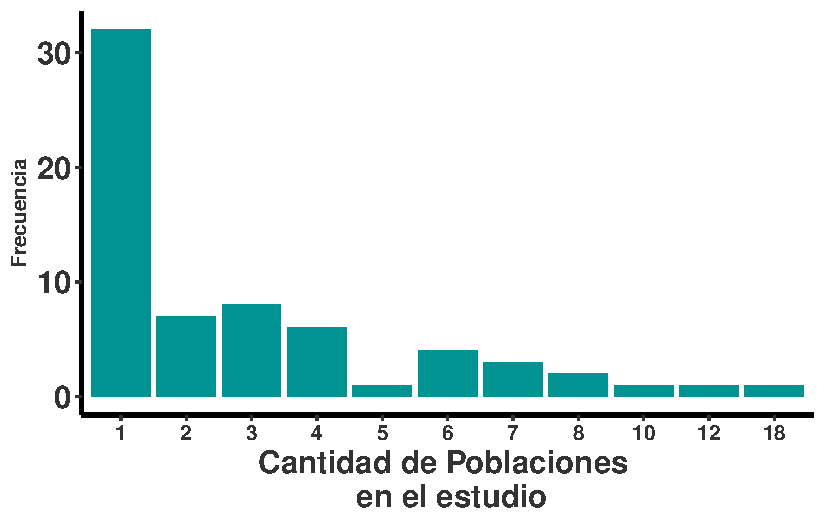
\includegraphics{120-Rage_orquideas_files/figure-pdf/Rage8-1.pdf}

\begin{center}\rule{0.5\linewidth}{0.5pt}\end{center}

\subsection{La cantidad de poblaciones por especies en la base de datos
de
COMPADRE.}\label{la-cantidad-de-poblaciones-por-especies-en-la-base-de-datos-de-compadre.}

La cantidad de poblaciones muestreadas por especie en la base de datos
de COMPADRE varía considerablemente. Aunque la mayoría de las especies
están representadas por una sola población, existen casos en los que se
han registrado hasta 20 poblaciones distintas para una misma especie.
Estas poblaciones pueden provenir de diferentes publicaciones
científicas o representar datos recolectados en distintos momentos o con
distintos objetivos dentro de una misma población. Por ejemplo, los
datos de \emph{Lepanthes rupestris} provienen de dos estudios
independientes (Tremblay \& Ackerman, 2001; Tremblay \& McCarthy, 2014).
En el primero, se utilizaron matrices poblacionales para estimar el
tamaño efectivo de las poblaciones (Ne), mientras que en el segundo se
emplearon los mismos datos para desarrollar un enfoque bayesiano que
permite estimar los elementos de las matrices de transición,
especialmente útil cuando se dispone de pocos datos por población o
periodo. Este enfoque aprovecha la información conjunta de todas las
poblaciones para generar estimaciones más robustas y biológicamente
realistas.

\begin{center}\rule{0.5\linewidth}{0.5pt}\end{center}

\subsection{¿Cuan largo fueron los
estudios?}\label{cuan-largo-fueron-los-estudios}

La duración de los estudios en la base de datos de orquídeas de COMPADRE
varía considerablemente. Aunque muchos estudios abarcan solo unos pocos
años ---el mínimo requerido para calcular una matriz de transición
poblacional es de dos periodos---, también existen investigaciones que
se extienden por lapsos más prolongados. Algunos estudios, como los
realizados por Tremblay con \emph{Lepanthes rupestris}, incluyen
muestreos mensuales, mientras que otros se basan en observaciones
anuales. Esta diversidad en la temporalidad refleja tanto los objetivos
específicos de cada investigación como las estrategias metodológicas
empleadas.

La siguiente visualización muestra cómo varía la duración de los
estudios según el tipo de orquídea, diferenciando entre especies
epífitas y terrestres:

\begin{Shaded}
\begin{Highlighting}[]
\NormalTok{SPECIES\_O}\SpecialCharTok{$}\NormalTok{SpeciesAccepted }\OtherTok{\textless{}{-}} \FunctionTok{fct\_reorder}\NormalTok{(}
\NormalTok{  SPECIES\_O}\SpecialCharTok{$}\NormalTok{SpeciesAccepted,}
\NormalTok{  SPECIES\_O}\SpecialCharTok{$}\NormalTok{StudyStart,}
  \AttributeTok{.desc =} \ConstantTok{FALSE}
\NormalTok{)}



\FunctionTok{ggplot}\NormalTok{(SPECIES\_O, }\FunctionTok{aes}\NormalTok{(SpeciesAccepted, }\AttributeTok{ymin =}\NormalTok{ StudyStart, }\AttributeTok{ymax =}\NormalTok{ StudyEnd, }\AttributeTok{color =}\NormalTok{ OrganismType\_RC)) }\SpecialCharTok{+}
  \FunctionTok{geom\_linerange}\NormalTok{() }\SpecialCharTok{+}
  \FunctionTok{coord\_flip}\NormalTok{() }\SpecialCharTok{+}
  \FunctionTok{theme}\NormalTok{(}\AttributeTok{legend.position.inside =} \FunctionTok{c}\NormalTok{(}\FloatTok{0.2}\NormalTok{, }\FloatTok{0.8}\NormalTok{)) }\SpecialCharTok{+}
  \FunctionTok{ylab}\NormalTok{(}\StringTok{""}\NormalTok{) }\SpecialCharTok{+}
  \FunctionTok{xlab}\NormalTok{(}\StringTok{""}\NormalTok{) }\SpecialCharTok{+}
  \FunctionTok{rlt\_style\_colour}\NormalTok{() }\SpecialCharTok{+}
  \FunctionTok{theme}\NormalTok{(}
    \AttributeTok{axis.text.x =} \FunctionTok{element\_text}\NormalTok{(}
      \AttributeTok{color =} \StringTok{"grey20"}\NormalTok{,}
      \AttributeTok{size =} \DecValTok{9}\NormalTok{,}
      \AttributeTok{angle =} \DecValTok{90}\NormalTok{,}
      \AttributeTok{hjust =}\NormalTok{ .}\DecValTok{5}\NormalTok{,}
      \AttributeTok{vjust =}\NormalTok{ .}\DecValTok{5}\NormalTok{,}
      \AttributeTok{face =} \StringTok{"plain"}
\NormalTok{    ),}
    \AttributeTok{axis.text.y =} \FunctionTok{element\_text}\NormalTok{(}
      \AttributeTok{color =} \StringTok{"grey20"}\NormalTok{,}
      \AttributeTok{size =} \DecValTok{7}\NormalTok{,}
      \AttributeTok{angle =} \DecValTok{0}\NormalTok{,}
      \AttributeTok{hjust =} \DecValTok{1}\NormalTok{,}
      \AttributeTok{vjust =} \DecValTok{0}\NormalTok{,}
      \AttributeTok{face =} \StringTok{"plain"}
\NormalTok{    ),}
    \AttributeTok{axis.title.x =} \FunctionTok{element\_text}\NormalTok{(}
      \AttributeTok{color =} \StringTok{"grey20"}\NormalTok{,}
      \AttributeTok{size =} \DecValTok{12}\NormalTok{,}
      \AttributeTok{angle =} \DecValTok{0}\NormalTok{,}
      \AttributeTok{hjust =}\NormalTok{ .}\DecValTok{5}\NormalTok{,}
      \AttributeTok{vjust =} \DecValTok{0}\NormalTok{,}
      \AttributeTok{face =} \StringTok{"plain"}
\NormalTok{    ),}
    \AttributeTok{axis.title.y =} \FunctionTok{element\_text}\NormalTok{(}
      \AttributeTok{color =} \StringTok{"grey20"}\NormalTok{,}
      \AttributeTok{size =} \DecValTok{12}\NormalTok{,}
      \AttributeTok{angle =} \DecValTok{90}\NormalTok{,}
      \AttributeTok{hjust =}\NormalTok{ .}\DecValTok{5}\NormalTok{,}
      \AttributeTok{vjust =}\NormalTok{ .}\DecValTok{5}\NormalTok{,}
      \AttributeTok{face =} \StringTok{"plain"}
\NormalTok{    )}
\NormalTok{  )}\SpecialCharTok{+}
  \FunctionTok{theme}\NormalTok{(}\AttributeTok{legend.position =} \FunctionTok{c}\NormalTok{(}\FloatTok{0.2}\NormalTok{,}\FloatTok{0.8}\NormalTok{),}
        \AttributeTok{legend.title =} \FunctionTok{element\_blank}\NormalTok{())}\SpecialCharTok{+}
  \FunctionTok{theme}\NormalTok{(}\AttributeTok{axis.text.y =} \FunctionTok{element\_text}\NormalTok{(}\AttributeTok{size =} \DecValTok{5}\NormalTok{))}\SpecialCharTok{+}
  \FunctionTok{scale\_y\_continuous}\NormalTok{(}\AttributeTok{n.breaks =} \DecValTok{12}\NormalTok{)}
\end{Highlighting}
\end{Shaded}

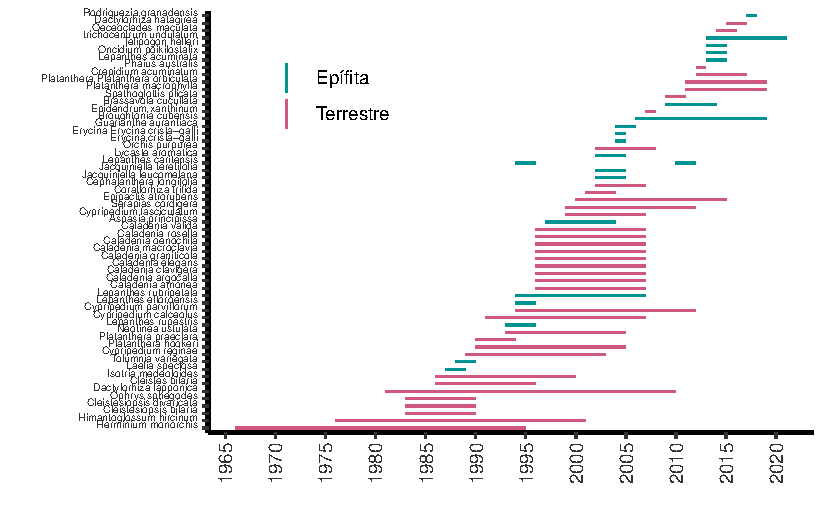
\includegraphics{120-Rage_orquideas_files/figure-pdf/Rage9-1.pdf}

\begin{Shaded}
\begin{Highlighting}[]
\CommentTok{\#ggsave("Figures/Lenght\_survey.png")}
\end{Highlighting}
\end{Shaded}

\begin{center}\rule{0.5\linewidth}{0.5pt}\end{center}

\subsection{Tiempo de duración de las
investigaciones.}\label{tiempo-de-duraciuxf3n-de-las-investigaciones.}

La siguiente figura muestra la duración de los estudios realizados sobre
orquídeas epífitas y terrestres. Según los datos extraídos de la base de
datos COMPADRE, la mayoría de las investigaciones tuvieron una duración
relativamente corta, especialmente en el caso de las especies epífitas.
Sin embargo, también se registran estudios que se extendieron por más de
20 años, lo que evidencia un compromiso a largo plazo en algunos casos
para entender mejor la dinámica poblacional de estas plantas.

\begin{Shaded}
\begin{Highlighting}[]
\NormalTok{Orquideas }\OtherTok{=}\NormalTok{ Orquideas }\SpecialCharTok{\%\textgreater{}\%}
  \FunctionTok{mutate}\NormalTok{(}\AttributeTok{StudyDuration =} \FunctionTok{as.numeric}\NormalTok{(StudyDuration),}
    \AttributeTok{OrganismType\_RC =} \FunctionTok{fct\_recode}\NormalTok{(}
\NormalTok{      OrganismType,}
      \StringTok{"Epífita"} \OtherTok{=} \StringTok{"Epiphyte"}\NormalTok{,}
      \StringTok{"Terrestre"} \OtherTok{=} \StringTok{"Herbaceous perennial"}
\NormalTok{    )}
\NormalTok{  )}


\CommentTok{\#table(Orquideas$StudyDuration)}
\CommentTok{\#table(Orquideas$OrganismType)}

\FunctionTok{ggplot}\NormalTok{(Orquideas, }\FunctionTok{aes}\NormalTok{(StudyDuration, }\AttributeTok{fill =}\NormalTok{ OrganismType\_RC)) }\SpecialCharTok{+}
  \FunctionTok{geom\_histogram}\NormalTok{(}\AttributeTok{colour =} \StringTok{"white"}\NormalTok{) }\SpecialCharTok{+}
  \FunctionTok{facet\_wrap}\NormalTok{(}\SpecialCharTok{\textasciitilde{}}\NormalTok{OrganismType\_RC) }\SpecialCharTok{+}
  \FunctionTok{theme}\NormalTok{(}\AttributeTok{legend.position =} \StringTok{"none"}\NormalTok{) }\SpecialCharTok{+}
  \FunctionTok{xlab}\NormalTok{(}\StringTok{"Duración de los estudios"}\NormalTok{) }\SpecialCharTok{+}
  \FunctionTok{ylab}\NormalTok{(}\StringTok{"Frecuencia"}\NormalTok{) }\SpecialCharTok{+}
  \FunctionTok{rlt\_style\_fill}\NormalTok{() }\SpecialCharTok{+}
  \FunctionTok{scale\_x\_continuous}\NormalTok{(}\AttributeTok{n.breaks =} \DecValTok{10}\NormalTok{)}
\end{Highlighting}
\end{Shaded}

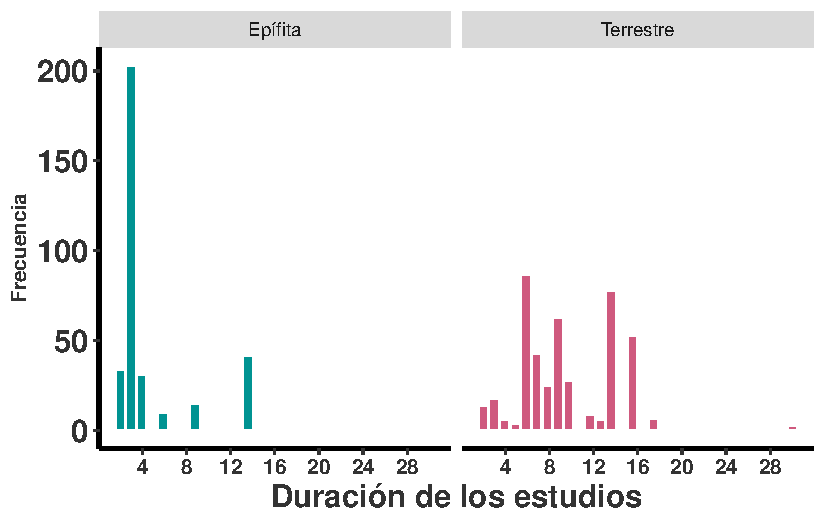
\includegraphics{120-Rage_orquideas_files/figure-pdf/Rage10-1.pdf}

\begin{Shaded}
\begin{Highlighting}[]
\CommentTok{\#ggsave("Duración\_Epi\_Ter.pdf")}

\FunctionTok{ggsave}\NormalTok{(}\StringTok{"Figures/Duración\_Epi\_Ter.png"}\NormalTok{)}
\end{Highlighting}
\end{Shaded}

\begin{center}\rule{0.5\linewidth}{0.5pt}\end{center}

\begin{center}\rule{0.5\linewidth}{0.5pt}\end{center}

\subsection{Cálculo del Valor Propio Dominante (λ) en Matrices Ergodicas
e
Irreductibles}\label{cuxe1lculo-del-valor-propio-dominante-ux3bb-en-matrices-ergodicas-e-irreductibles}

A partir del conjunto de matrices previamente filtradas por cumplir con
las condiciones de ergodicidad e irreducibilidad, se procede al cálculo
del valor propio dominante (\(\lambda\)), el cual representa la tasa de
crecimiento poblacional asintótica en modelos matriciales.

Para ello, se emplea la función eigs del paquete popdemo, que permite
obtener los valores propios de una matriz. Esta función se aplica a cada
matriz seleccionada mediante sapply, generando una lista de valores de
(\(\lambda\)) almacenados en el objeto lambdaVals. Cada entrada en esta
lista corresponde al valor propio dominante de una matriz matA incluida
en el conjunto de datos.

Posteriormente, se utiliza la función summary para obtener una
descripción estadística de los valores de (\(\lambda\)), y la función
hist para visualizar su distribución, lo que permite evaluar la
variabilidad en las tasas de crecimiento poblacional entre las distintas
especies o poblaciones representadas.

\subsubsection{Matrices ergódicas e
irreductibles}\label{matrices-erguxf3dicas-e-irreductibles}

\begin{Shaded}
\begin{Highlighting}[]
\NormalTok{Compadre\_flagged }\OtherTok{\textless{}{-}} \FunctionTok{cdb\_flag}\NormalTok{(Orquideas)}


\NormalTok{Mat\_erg\_irred }\OtherTok{\textless{}{-}} \FunctionTok{subset}\NormalTok{(}
\NormalTok{  Compadre\_flagged,}
\NormalTok{  check\_NA\_A }\SpecialCharTok{==} \ConstantTok{FALSE} \SpecialCharTok{\&}\NormalTok{ check\_irreducible }\SpecialCharTok{==} \ConstantTok{TRUE} \SpecialCharTok{\&}\NormalTok{ check\_ergodic }\SpecialCharTok{==} \ConstantTok{TRUE}
\NormalTok{) }\CommentTok{\# para evaluar si las matrices son ergódicas e irreducibles al mismo tiempo}

\FunctionTok{head}\NormalTok{(}\FunctionTok{cdb\_metadata}\NormalTok{(Mat\_erg\_irred), }\AttributeTok{n=}\DecValTok{2}\NormalTok{) }\SpecialCharTok{|\textgreater{}} 
  \FunctionTok{gt}\NormalTok{()}
\end{Highlighting}
\end{Shaded}

\begin{table}
\fontsize{12.0pt}{14.0pt}\selectfont
\begin{tabular*}{\linewidth}{@{\extracolsep{\fill}}rlllllllllllllllllllrllrrrrllllrrrrllllllllrlrrlrllllrrlllccccccccccccccc}
\toprule
MatrixID & SpeciesAuthor & SpeciesAccepted & CommonName & Kingdom & Phylum & Class & Order & Family & Genus & Species & Infraspecies & InfraspeciesType & OrganismType & DicotMonoc & AngioGymno & Authors & Journal & SourceType & OtherType & YearPublication & DOI\_ISBN & AdditionalSource & StudyDuration & StudyStart & StudyEnd & ProjectionInterval & MatrixCriteriaSize & MatrixCriteriaOntogeny & MatrixCriteriaAge & MatrixPopulation & NumberPopulations & Lat & Lon & Altitude & Country & Continent & Ecoregion & StudiedSex & MatrixComposite & MatrixSeasonal & MatrixTreatment & MatrixCaptivity & MatrixStartYear & MatrixStartSeason & MatrixStartMonth & MatrixEndYear & MatrixEndSeason & MatrixEndMonth & CensusType & MatrixSplit & MatrixFec & Observations & MatrixDimension & SurvivalIssue & \_Database & \_PopulationStatus & \_PublicationStatus & OrganismType\_RC & check\_NA\_A & check\_NA\_U & check\_NA\_F & check\_NA\_C & check\_zero\_U & check\_zero\_F & check\_zero\_C & check\_zero\_U\_colsum & check\_singular\_U & check\_component\_sum & check\_ergodic & check\_irreducible & check\_primitive & check\_surv\_gte\_1 \\ 
\midrule\addlinespace[2.5pt]
238285 & Caladenia\_amonea & Caladenia amonea & NA & Plantae & Tracheophyta & Liliopsida & Asparagales & Orchidaceae & Caladenia & amonea & NA & NA & Herbaceous perennial & Monocot & Angiosperm & Raymond L. Tremblay; P\\'erez; Larcombe; Brown; Quarmby; Bickerton; French; Bould & Aust J Bot & Journal Article & NA & 2009 & 10.1071/BT08167 & NA & 12 & 1996 & 2007 & 1 & No & Yes & No & North-eastern Melbourne, Vic & 1 & NA & NA & NA & AUS & Oceania & TBM & A & Mean & No & Unmanipulated & W & 1996 & Summer & 8 & 2007 & Autumn & 9 & NA & Divided & NA & Locations of surveyed areas are kept vague to reduce the likelihood of unauthorised disturbance of the populations & 3 & 1 & COMPADRE & Released & Released & Terrestre & FALSE & FALSE & FALSE & FALSE & FALSE & TRUE & TRUE & FALSE & FALSE & TRUE & TRUE & TRUE & TRUE & FALSE \\ 
238286 & Caladenia\_argocalla & Caladenia argocalla & NA & Plantae & Tracheophyta & Liliopsida & Asparagales & Orchidaceae & Caladenia & argocalla & NA & NA & Herbaceous perennial & Monocot & Angiosperm & Raymond L. Tremblay; P\\'erez; Larcombe; Brown; Quarmby; Bickerton; French; Bould & Aust J Bot & Journal Article & NA & 2009 & 10.1071/BT08167 & NA & 12 & 1996 & 2007 & 1 & No & Yes & No & Adelaide Hills and Clare Valley, SA & 1 & NA & NA & NA & AUS & Oceania & TBM & A & Mean & No & Unmanipulated & W & 2003 & Autumn & 9 & 2007 & Autumn & 10 & NA & Divided & No & Locations of surveyed areas are kept vague to reduce the likelihood of unauthorised disturbance of the populations & 3 & 1 & COMPADRE & Released & Released & Terrestre & FALSE & FALSE & FALSE & FALSE & FALSE & TRUE & TRUE & FALSE & FALSE & TRUE & TRUE & TRUE & TRUE & FALSE \\ 
\bottomrule
\end{tabular*}
\end{table}

\begin{Shaded}
\begin{Highlighting}[]
\NormalTok{lambdaVals\_list }\OtherTok{\textless{}{-}} \FunctionTok{sapply}\NormalTok{(}\FunctionTok{matA}\NormalTok{(Mat\_erg\_irred), popdemo}\SpecialCharTok{::}\NormalTok{eigs, }\AttributeTok{what =} \StringTok{"lambda"}\NormalTok{) }



\NormalTok{lambdaVals}\OtherTok{=}\FunctionTok{as\_tibble}\NormalTok{(lambdaVals\_list)}

\FunctionTok{tidy}\NormalTok{(lambdaVals) }\SpecialCharTok{|\textgreater{}} \FunctionTok{gt}\NormalTok{()}
\end{Highlighting}
\end{Shaded}

\begin{table}
\fontsize{12.0pt}{14.0pt}\selectfont
\begin{tabular*}{\linewidth}{@{\extracolsep{\fill}}lrrrrrrrrrrrr}
\toprule
column & n & mean & sd & median & trimmed & mad & min & max & range & skew & kurtosis & se \\ 
\midrule\addlinespace[2.5pt]
value & 491 & 0.9835195 & 0.1378241 & 0.9939963 & 0.9862572 & 0.04496007 & 0.3887968 & 1.776031 & 1.387234 & -0.2986587 & 9.917098 & 0.006219916 \\ 
\bottomrule
\end{tabular*}
\end{table}

\begin{Shaded}
\begin{Highlighting}[]
\FunctionTok{ggplot}\NormalTok{(lambdaVals, }\FunctionTok{aes}\NormalTok{(value))}\SpecialCharTok{+}
  \FunctionTok{geom\_histogram}\NormalTok{(}\FunctionTok{aes}\NormalTok{(}\AttributeTok{fill=}\StringTok{"lightblue"}\NormalTok{), }\AttributeTok{colour=}\StringTok{"white"}\NormalTok{)}\SpecialCharTok{+}
  \FunctionTok{rlt\_style\_fill}\NormalTok{()}\SpecialCharTok{+}
  \FunctionTok{xlab}\NormalTok{(}\StringTok{"Lambda"}\NormalTok{)}\SpecialCharTok{+}
  \FunctionTok{ylab}\NormalTok{(}\StringTok{"Frecuencia"}\NormalTok{)}\SpecialCharTok{+}
  \FunctionTok{scale\_x\_continuous}\NormalTok{(}\AttributeTok{n.breaks =} \DecValTok{10}\NormalTok{)}\SpecialCharTok{+}
  \FunctionTok{theme}\NormalTok{(}\AttributeTok{legend.position =} \StringTok{"none"}\NormalTok{)}
\end{Highlighting}
\end{Shaded}

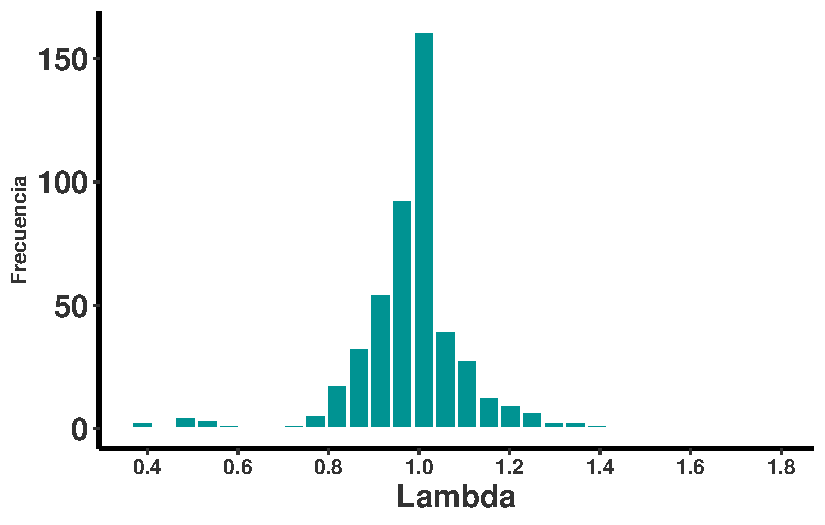
\includegraphics{120-Rage_orquideas_files/figure-pdf/Rage13-1.pdf}

Una metodología alternativa para calcular los valores propios dominantes
(\(\lambda\)) de las matrices de transición poblacional consiste en
utilizar la función \texttt{map\_dbl} de la librería purrr. Esta función
permite aplicar una operación a cada elemento de una lista, devolviendo
un vector numérico de igual longitud. En este contexto, se aplica una
función de cálculo de \(\lambda\) a cada matriz de transición (matA),
obteniendo así un valor de \(\lambda\) por matriz. Esta estrategia
resulta eficiente para el procesamiento simultáneo de múltiples matrices
dentro de un flujo de trabajo reproducible en R.

\begin{Shaded}
\begin{Highlighting}[]
\DocumentationTok{\#\# con el paquete popdemo}
\NormalTok{lambdaVals1 }\OtherTok{\textless{}{-}} \FunctionTok{map\_dbl}\NormalTok{(}
  \FunctionTok{matA}\NormalTok{(Mat\_erg\_irred),}
  \SpecialCharTok{\textasciitilde{}}\NormalTok{ popdemo}\SpecialCharTok{::}\FunctionTok{eigs}\NormalTok{(.x, }\AttributeTok{what =} \StringTok{"lambda"}\NormalTok{)}
\NormalTok{)}


\DocumentationTok{\#\# O puede calcular lambda con el paquete popbio, que evita algunos mensajes de advertencia}

\NormalTok{lambdaVals2 }\OtherTok{\textless{}{-}} \FunctionTok{map\_dbl}\NormalTok{(}\FunctionTok{matA}\NormalTok{(Mat\_erg\_irred), }\SpecialCharTok{\textasciitilde{}}\NormalTok{ popbio}\SpecialCharTok{::}\FunctionTok{lambda}\NormalTok{(.x))}
\end{Highlighting}
\end{Shaded}

\begin{center}\rule{0.5\linewidth}{0.5pt}\end{center}

\section{Variación en el crecimiento poblacional entre especies epífitas
y
terrestres}\label{variaciuxf3n-en-el-crecimiento-poblacional-entre-especies-epuxedfitas-y-terrestres}

En esta sección se seleccionan las especies clasificadas como epífitas y
terrestres, agrupándolas en objetos distintos que contienen todas las
poblaciones muestreadas correspondientes. Esta separación permite
evaluar comparativamente la variación en las tasas de crecimiento
poblacional entre ambos grupos funcionales, facilitando el análisis de
patrones ecológicos y demográficos asociados a sus respectivos hábitos
de vida.

\begin{Shaded}
\begin{Highlighting}[]
\NormalTok{epifitas }\OtherTok{=}\NormalTok{ Orquideas }\SpecialCharTok{\%\textgreater{}\%}
  \FunctionTok{filter}\NormalTok{(OrganismType }\SpecialCharTok{==} \StringTok{"Epiphyte"}\NormalTok{)}

\NormalTok{terrestres }\OtherTok{=}\NormalTok{ Orquideas }\SpecialCharTok{\%\textgreater{}\%}
  \FunctionTok{filter}\NormalTok{(OrganismType }\SpecialCharTok{==} \StringTok{"Herbaceous perennial"}\NormalTok{)}
\end{Highlighting}
\end{Shaded}

\begin{Shaded}
\begin{Highlighting}[]
\NormalTok{Compadre\_flagged\_epif }\OtherTok{\textless{}{-}} \FunctionTok{cdb\_flag}\NormalTok{(epifitas)}

\NormalTok{x\_epif }\OtherTok{\textless{}{-}} \FunctionTok{subset}\NormalTok{(}
\NormalTok{  Compadre\_flagged\_epif,}
\NormalTok{  check\_NA\_A }\SpecialCharTok{==} \ConstantTok{FALSE} \SpecialCharTok{\&}\NormalTok{ check\_ergodic }\SpecialCharTok{==} \ConstantTok{TRUE}
\NormalTok{)}

\CommentTok{\#sapply(matA(x\_epi), popdemo::eigs, what="lambda")}

\NormalTok{lambda\_epif }\OtherTok{\textless{}{-}} \FunctionTok{map\_dbl}\NormalTok{(}\FunctionTok{matA}\NormalTok{(x\_epif), }\SpecialCharTok{\textasciitilde{}}\NormalTok{ popdemo}\SpecialCharTok{::}\FunctionTok{eigs}\NormalTok{(.x, }\AttributeTok{what =} \StringTok{"lambda"}\NormalTok{))}

\CommentTok{\#Or with popbio, which avoids some warning messages…}

\NormalTok{Compadre\_flagged\_terrestres }\OtherTok{\textless{}{-}} \FunctionTok{cdb\_flag}\NormalTok{(terrestres)}


\NormalTok{x\_terr }\OtherTok{\textless{}{-}} \FunctionTok{subset}\NormalTok{(}
\NormalTok{  Compadre\_flagged\_terrestres,}
\NormalTok{  check\_NA\_A }\SpecialCharTok{==} \ConstantTok{FALSE} \SpecialCharTok{\&}\NormalTok{ check\_ergodic }\SpecialCharTok{==} \ConstantTok{TRUE}
\NormalTok{)}



\NormalTok{lambda\_terr }\OtherTok{\textless{}{-}} \FunctionTok{map\_dbl}\NormalTok{(}\FunctionTok{matA}\NormalTok{(x\_terr), }\SpecialCharTok{\textasciitilde{}}\NormalTok{ popdemo}\SpecialCharTok{::}\FunctionTok{eigs}\NormalTok{(.x, }\AttributeTok{what =} \StringTok{"lambda"}\NormalTok{))}
\end{Highlighting}
\end{Shaded}

\begin{center}\rule{0.5\linewidth}{0.5pt}\end{center}

\subsection{Evaluación de Tendencias Centrales y Dispersión en Especies
Terrestres y
Epífitas}\label{evaluaciuxf3n-de-tendencias-centrales-y-dispersiuxf3n-en-especies-terrestres-y-epuxedfitas}

Mediante el uso de la función summary, se analizaron las medidas de
tendencia central y dispersión de los valores propios de lambda
correspondientes a especies terrestres y epífitas. Los resultados
indican que las especies terrestres presentan una mayor dispersión en
los valores de lambda en comparación con las especies epífitas. Aunque
los promedios difieren ligeramente entre ambos grupos, las medianas
resultaron ser similares, lo que sugiere patrones demográficos
comparables en términos de centralidad, pero con variabilidad distinta
en su comportamiento poblacional.

\begin{Shaded}
\begin{Highlighting}[]
\FunctionTok{library}\NormalTok{(flextable)}

\CommentTok{\# Clacular resúmenes}
\NormalTok{epif\_summary }\OtherTok{\textless{}{-}} \FunctionTok{summary}\NormalTok{(lambda\_epif)}
\NormalTok{terr\_summary }\OtherTok{\textless{}{-}} \FunctionTok{summary}\NormalTok{(lambda\_terr)}

\CommentTok{\# Unire los resúmenes en un solo data frame}
\NormalTok{combined\_df }\OtherTok{\textless{}{-}} \FunctionTok{rbind}\NormalTok{(}
\NormalTok{  Epífita }\OtherTok{=}\NormalTok{ epif\_summary,}
  \AttributeTok{Terrestre =}\NormalTok{ terr\_summary}
\NormalTok{)}

\CommentTok{\# Convertir a data frame y añadir columna de hábitat}
\NormalTok{combined\_df }\OtherTok{\textless{}{-}} \FunctionTok{as.data.frame}\NormalTok{(combined\_df)}
\NormalTok{combined\_df}\SpecialCharTok{$}\NormalTok{Habit }\OtherTok{\textless{}{-}} \FunctionTok{rownames}\NormalTok{(combined\_df)}

\CommentTok{\# Reordenar columnas}
\NormalTok{combined\_df }\OtherTok{\textless{}{-}}\NormalTok{ combined\_df[, }\FunctionTok{c}\NormalTok{(}\StringTok{"Habit"}\NormalTok{, }\FunctionTok{names}\NormalTok{(epif\_summary))]}

\CommentTok{\# Crear la tabla con flextable}
\FunctionTok{flextable}\NormalTok{(combined\_df) }\SpecialCharTok{|\textgreater{}}
  \FunctionTok{autofit}\NormalTok{() }\SpecialCharTok{|\textgreater{}}
  \FunctionTok{theme\_vanilla}\NormalTok{()}
\end{Highlighting}
\end{Shaded}

\global\setlength{\Oldarrayrulewidth}{\arrayrulewidth}

\global\setlength{\Oldtabcolsep}{\tabcolsep}

\setlength{\tabcolsep}{2pt}

\renewcommand*{\arraystretch}{1.5}



\providecommand{\ascline}[3]{\noalign{\global\arrayrulewidth #1}\arrayrulecolor[HTML]{#2}\cline{#3}}

\begin{longtable*}[c]{|p{0.90in}|p{1.01in}|p{1.01in}|p{1.01in}|p{1.01in}|p{0.92in}|p{0.92in}}



\ascline{1.5pt}{666666}{1-7}

\multicolumn{1}{>{\raggedright}m{\dimexpr 0.9in+0\tabcolsep}}{\textcolor[HTML]{000000}{\fontsize{11}{11}\selectfont{\global\setmainfont{Helvetica}{\textbf{Habit}}}}} & \multicolumn{1}{>{\raggedleft}m{\dimexpr 1.01in+0\tabcolsep}}{\textcolor[HTML]{000000}{\fontsize{11}{11}\selectfont{\global\setmainfont{Helvetica}{\textbf{Min.}}}}} & \multicolumn{1}{>{\raggedleft}m{\dimexpr 1.01in+0\tabcolsep}}{\textcolor[HTML]{000000}{\fontsize{11}{11}\selectfont{\global\setmainfont{Helvetica}{\textbf{1st\ Qu.}}}}} & \multicolumn{1}{>{\raggedleft}m{\dimexpr 1.01in+0\tabcolsep}}{\textcolor[HTML]{000000}{\fontsize{11}{11}\selectfont{\global\setmainfont{Helvetica}{\textbf{Median}}}}} & \multicolumn{1}{>{\raggedleft}m{\dimexpr 1.01in+0\tabcolsep}}{\textcolor[HTML]{000000}{\fontsize{11}{11}\selectfont{\global\setmainfont{Helvetica}{\textbf{Mean}}}}} & \multicolumn{1}{>{\raggedleft}m{\dimexpr 0.92in+0\tabcolsep}}{\textcolor[HTML]{000000}{\fontsize{11}{11}\selectfont{\global\setmainfont{Helvetica}{\textbf{3rd\ Qu.}}}}} & \multicolumn{1}{>{\raggedleft}m{\dimexpr 0.92in+0\tabcolsep}}{\textcolor[HTML]{000000}{\fontsize{11}{11}\selectfont{\global\setmainfont{Helvetica}{\textbf{Max.}}}}} \\

\ascline{1.5pt}{666666}{1-7}\endfirsthead 

\ascline{1.5pt}{666666}{1-7}

\multicolumn{1}{>{\raggedright}m{\dimexpr 0.9in+0\tabcolsep}}{\textcolor[HTML]{000000}{\fontsize{11}{11}\selectfont{\global\setmainfont{Helvetica}{\textbf{Habit}}}}} & \multicolumn{1}{>{\raggedleft}m{\dimexpr 1.01in+0\tabcolsep}}{\textcolor[HTML]{000000}{\fontsize{11}{11}\selectfont{\global\setmainfont{Helvetica}{\textbf{Min.}}}}} & \multicolumn{1}{>{\raggedleft}m{\dimexpr 1.01in+0\tabcolsep}}{\textcolor[HTML]{000000}{\fontsize{11}{11}\selectfont{\global\setmainfont{Helvetica}{\textbf{1st\ Qu.}}}}} & \multicolumn{1}{>{\raggedleft}m{\dimexpr 1.01in+0\tabcolsep}}{\textcolor[HTML]{000000}{\fontsize{11}{11}\selectfont{\global\setmainfont{Helvetica}{\textbf{Median}}}}} & \multicolumn{1}{>{\raggedleft}m{\dimexpr 1.01in+0\tabcolsep}}{\textcolor[HTML]{000000}{\fontsize{11}{11}\selectfont{\global\setmainfont{Helvetica}{\textbf{Mean}}}}} & \multicolumn{1}{>{\raggedleft}m{\dimexpr 0.92in+0\tabcolsep}}{\textcolor[HTML]{000000}{\fontsize{11}{11}\selectfont{\global\setmainfont{Helvetica}{\textbf{3rd\ Qu.}}}}} & \multicolumn{1}{>{\raggedleft}m{\dimexpr 0.92in+0\tabcolsep}}{\textcolor[HTML]{000000}{\fontsize{11}{11}\selectfont{\global\setmainfont{Helvetica}{\textbf{Max.}}}}} \\

\ascline{1.5pt}{666666}{1-7}\endhead



\multicolumn{1}{>{\raggedright}m{\dimexpr 0.9in+0\tabcolsep}}{\textcolor[HTML]{000000}{\fontsize{11}{11}\selectfont{\global\setmainfont{Helvetica}{Epífita}}}} & \multicolumn{1}{>{\raggedleft}m{\dimexpr 1.01in+0\tabcolsep}}{\textcolor[HTML]{000000}{\fontsize{11}{11}\selectfont{\global\setmainfont{Helvetica}{0.3887968}}}} & \multicolumn{1}{>{\raggedleft}m{\dimexpr 1.01in+0\tabcolsep}}{\textcolor[HTML]{000000}{\fontsize{11}{11}\selectfont{\global\setmainfont{Helvetica}{0.9690608}}}} & \multicolumn{1}{>{\raggedleft}m{\dimexpr 1.01in+0\tabcolsep}}{\textcolor[HTML]{000000}{\fontsize{11}{11}\selectfont{\global\setmainfont{Helvetica}{0.9950628}}}} & \multicolumn{1}{>{\raggedleft}m{\dimexpr 1.01in+0\tabcolsep}}{\textcolor[HTML]{000000}{\fontsize{11}{11}\selectfont{\global\setmainfont{Helvetica}{0.9776130}}}} & \multicolumn{1}{>{\raggedleft}m{\dimexpr 0.92in+0\tabcolsep}}{\textcolor[HTML]{000000}{\fontsize{11}{11}\selectfont{\global\setmainfont{Helvetica}{1.004671}}}} & \multicolumn{1}{>{\raggedleft}m{\dimexpr 0.92in+0\tabcolsep}}{\textcolor[HTML]{000000}{\fontsize{11}{11}\selectfont{\global\setmainfont{Helvetica}{1.359231}}}} \\

\ascline{0.75pt}{666666}{1-7}



\multicolumn{1}{>{\raggedright}m{\dimexpr 0.9in+0\tabcolsep}}{\textcolor[HTML]{000000}{\fontsize{11}{11}\selectfont{\global\setmainfont{Helvetica}{Terrestre}}}} & \multicolumn{1}{>{\raggedleft}m{\dimexpr 1.01in+0\tabcolsep}}{\textcolor[HTML]{000000}{\fontsize{11}{11}\selectfont{\global\setmainfont{Helvetica}{0.4088863}}}} & \multicolumn{1}{>{\raggedleft}m{\dimexpr 1.01in+0\tabcolsep}}{\textcolor[HTML]{000000}{\fontsize{11}{11}\selectfont{\global\setmainfont{Helvetica}{0.9295530}}}} & \multicolumn{1}{>{\raggedleft}m{\dimexpr 1.01in+0\tabcolsep}}{\textcolor[HTML]{000000}{\fontsize{11}{11}\selectfont{\global\setmainfont{Helvetica}{0.9992454}}}} & \multicolumn{1}{>{\raggedleft}m{\dimexpr 1.01in+0\tabcolsep}}{\textcolor[HTML]{000000}{\fontsize{11}{11}\selectfont{\global\setmainfont{Helvetica}{0.9988654}}}} & \multicolumn{1}{>{\raggedleft}m{\dimexpr 0.92in+0\tabcolsep}}{\textcolor[HTML]{000000}{\fontsize{11}{11}\selectfont{\global\setmainfont{Helvetica}{1.043194}}}} & \multicolumn{1}{>{\raggedleft}m{\dimexpr 0.92in+0\tabcolsep}}{\textcolor[HTML]{000000}{\fontsize{11}{11}\selectfont{\global\setmainfont{Helvetica}{1.776031}}}} \\

\ascline{1.5pt}{666666}{1-7}



\end{longtable*}



\arrayrulecolor[HTML]{000000}

\global\setlength{\arrayrulewidth}{\Oldarrayrulewidth}

\global\setlength{\tabcolsep}{\Oldtabcolsep}

\renewcommand*{\arraystretch}{1}

Para visualizar los datos en una figura de \textbf{ggplot2}, hay que
convertir estas filas en un data.frame y añadir una columna con el tipo
de habitad, renombrar la columna lambda y unir los dos data.frames en
uno solo.

\begin{Shaded}
\begin{Highlighting}[]
\NormalTok{df\_Lamb\_epif }\OtherTok{=} \FunctionTok{as.data.frame}\NormalTok{(lambda\_epif)}
\NormalTok{df\_Lamb\_terr }\OtherTok{=} \FunctionTok{as.data.frame}\NormalTok{(lambda\_terr)}
\end{Highlighting}
\end{Shaded}

Crear una columna con el tipo de hábitat y renombrar la columna lambda

\begin{Shaded}
\begin{Highlighting}[]
\NormalTok{df\_Lamb\_epi }\OtherTok{=}\NormalTok{ df\_Lamb\_epif }\SpecialCharTok{\%\textgreater{}\%}
  \FunctionTok{add\_column}\NormalTok{(}\AttributeTok{Habit\_Type =} \StringTok{"Epífitas"}\NormalTok{) }\SpecialCharTok{\%\textgreater{}\%}
  \FunctionTok{rename}\NormalTok{(}\AttributeTok{lambda =}\NormalTok{ lambda\_epif)}


\NormalTok{df\_Lamb\_terr }\OtherTok{=} \FunctionTok{as.data.frame}\NormalTok{(lambda\_terr)}
\NormalTok{df\_Lamb\_terr }\OtherTok{=}\NormalTok{ df\_Lamb\_terr }\SpecialCharTok{\%\textgreater{}\%}
  \FunctionTok{add\_column}\NormalTok{(}\AttributeTok{Habit\_Type =} \StringTok{"Terrestre"}\NormalTok{) }\SpecialCharTok{\%\textgreater{}\%}
  \FunctionTok{rename}\NormalTok{(}\AttributeTok{lambda =}\NormalTok{ lambda\_terr)}
\end{Highlighting}
\end{Shaded}

Unir los dos data.frame en uno solo

\begin{Shaded}
\begin{Highlighting}[]
\NormalTok{ALL\_Lambdas }\OtherTok{=} \FunctionTok{rbind}\NormalTok{(df\_Lamb\_epi, df\_Lamb\_terr) }\CommentTok{\# unir los dos data frame en uno}
\end{Highlighting}
\end{Shaded}

Visualizar el crecimiento poblacional por tipo de hábitat

\begin{Shaded}
\begin{Highlighting}[]
\FunctionTok{ggplot}\NormalTok{(ALL\_Lambdas, }\FunctionTok{aes}\NormalTok{(lambda, }\AttributeTok{fill =}\NormalTok{ Habit\_Type)) }\SpecialCharTok{+}
  \FunctionTok{geom\_histogram}\NormalTok{(}\AttributeTok{colour =} \StringTok{"white"}\NormalTok{) }\SpecialCharTok{+}
  \FunctionTok{facet\_wrap}\NormalTok{(}\SpecialCharTok{\textasciitilde{}}\NormalTok{Habit\_Type) }\SpecialCharTok{+}
  \FunctionTok{rlt\_style\_fill}\NormalTok{()}\SpecialCharTok{+}
  \FunctionTok{scale\_x\_continuous}\NormalTok{(}\AttributeTok{n.breaks =} \DecValTok{8}\NormalTok{)}\SpecialCharTok{+}
  \FunctionTok{theme}\NormalTok{(}\AttributeTok{axis.text.x =} \FunctionTok{element\_text}\NormalTok{(}\AttributeTok{angle =} \DecValTok{45}\NormalTok{, }\AttributeTok{hjust =} \DecValTok{1}\NormalTok{))}\SpecialCharTok{+}
  \FunctionTok{ylab}\NormalTok{(}\StringTok{"Frecuencia"}\NormalTok{)}
\end{Highlighting}
\end{Shaded}

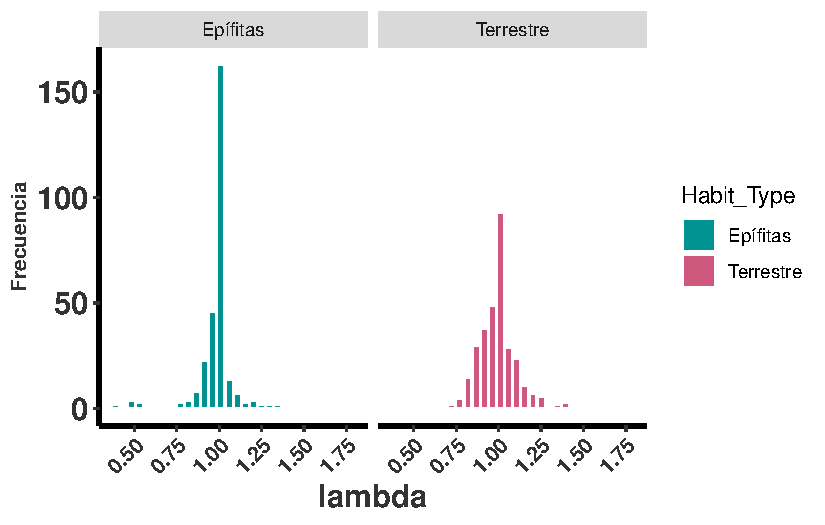
\includegraphics{120-Rage_orquideas_files/figure-pdf/Rage29-1.pdf}

\begin{Shaded}
\begin{Highlighting}[]
\CommentTok{\# ggsave("Figures/Terr\_Epi\_lambda.png")}
\end{Highlighting}
\end{Shaded}

\begin{center}\rule{0.5\linewidth}{0.5pt}\end{center}

\section{Estimación del crecimiento promedio y evaluación de diferencias
significativas}\label{estimaciuxf3n-del-crecimiento-promedio-y-evaluaciuxf3n-de-diferencias-significativas}

Para evaluar si existen diferencias significativas en los valores
propios de lambda entre especies epífitas y terrestres, se emplea un
modelo lineal utilizando la función \texttt{lm}. En este análisis, la
variable \textbf{Habit\_Type} se utiliza como predictor del valor propio
dominante (\(\lambda\)), lo que permite estimar el efecto del tipo de
hábitat sobre la tasa de crecimiento poblacional. Los resultados del
modelo indican que las especies epífitas tienden a presentar valores de
lambda más bajos en comparación con las especies terrestres. Para
obtener los coeficientes específicos de cada grupo, se ajusta un segundo
modelo excluyendo el intercepto mediante la inclusión de \texttt{-1} en
la fórmula. Esta parametrización permite calcular directamente el
promedio de lambda para cada grupo funcional, facilitando la comparación
entre ellos.

\begin{Shaded}
\begin{Highlighting}[]
\NormalTok{model\_lambda }\OtherTok{=} \FunctionTok{lm}\NormalTok{(lambda }\SpecialCharTok{\textasciitilde{}}\NormalTok{ Habit\_Type, }\AttributeTok{data =}\NormalTok{ ALL\_Lambdas)}
\CommentTok{\#summary(model\_lambda)}




\NormalTok{model\_lambda\_epi\_terr }\OtherTok{=} \FunctionTok{lm}\NormalTok{(lambda }\SpecialCharTok{\textasciitilde{}}\NormalTok{ Habit\_Type}\DecValTok{{-}1}\NormalTok{, }\AttributeTok{data =}\NormalTok{ ALL\_Lambdas)}
\CommentTok{\#summary(model\_lambda\_epi\_terr)}

\NormalTok{tidy\_results}\OtherTok{=} \FunctionTok{tidy}\NormalTok{(model\_lambda\_epi\_terr)}

\FunctionTok{flextable}\NormalTok{(tidy\_results)}
\end{Highlighting}
\end{Shaded}

\global\setlength{\Oldarrayrulewidth}{\arrayrulewidth}

\global\setlength{\Oldtabcolsep}{\tabcolsep}

\setlength{\tabcolsep}{2pt}

\renewcommand*{\arraystretch}{1.5}



\providecommand{\ascline}[3]{\noalign{\global\arrayrulewidth #1}\arrayrulecolor[HTML]{#2}\cline{#3}}

\begin{longtable*}[c]{|p{0.75in}|p{0.75in}|p{0.75in}|p{0.75in}|p{0.75in}}



\ascline{1.5pt}{666666}{1-5}

\multicolumn{1}{>{\raggedright}m{\dimexpr 0.75in+0\tabcolsep}}{\textcolor[HTML]{000000}{\fontsize{11}{11}\selectfont{\global\setmainfont{Helvetica}{term}}}} & \multicolumn{1}{>{\raggedleft}m{\dimexpr 0.75in+0\tabcolsep}}{\textcolor[HTML]{000000}{\fontsize{11}{11}\selectfont{\global\setmainfont{Helvetica}{estimate}}}} & \multicolumn{1}{>{\raggedleft}m{\dimexpr 0.75in+0\tabcolsep}}{\textcolor[HTML]{000000}{\fontsize{11}{11}\selectfont{\global\setmainfont{Helvetica}{std.error}}}} & \multicolumn{1}{>{\raggedleft}m{\dimexpr 0.75in+0\tabcolsep}}{\textcolor[HTML]{000000}{\fontsize{11}{11}\selectfont{\global\setmainfont{Helvetica}{statistic}}}} & \multicolumn{1}{>{\raggedleft}m{\dimexpr 0.75in+0\tabcolsep}}{\textcolor[HTML]{000000}{\fontsize{11}{11}\selectfont{\global\setmainfont{Helvetica}{p.value}}}} \\

\ascline{1.5pt}{666666}{1-5}\endfirsthead 

\ascline{1.5pt}{666666}{1-5}

\multicolumn{1}{>{\raggedright}m{\dimexpr 0.75in+0\tabcolsep}}{\textcolor[HTML]{000000}{\fontsize{11}{11}\selectfont{\global\setmainfont{Helvetica}{term}}}} & \multicolumn{1}{>{\raggedleft}m{\dimexpr 0.75in+0\tabcolsep}}{\textcolor[HTML]{000000}{\fontsize{11}{11}\selectfont{\global\setmainfont{Helvetica}{estimate}}}} & \multicolumn{1}{>{\raggedleft}m{\dimexpr 0.75in+0\tabcolsep}}{\textcolor[HTML]{000000}{\fontsize{11}{11}\selectfont{\global\setmainfont{Helvetica}{std.error}}}} & \multicolumn{1}{>{\raggedleft}m{\dimexpr 0.75in+0\tabcolsep}}{\textcolor[HTML]{000000}{\fontsize{11}{11}\selectfont{\global\setmainfont{Helvetica}{statistic}}}} & \multicolumn{1}{>{\raggedleft}m{\dimexpr 0.75in+0\tabcolsep}}{\textcolor[HTML]{000000}{\fontsize{11}{11}\selectfont{\global\setmainfont{Helvetica}{p.value}}}} \\

\ascline{1.5pt}{666666}{1-5}\endhead



\multicolumn{1}{>{\raggedright}m{\dimexpr 0.75in+0\tabcolsep}}{\textcolor[HTML]{000000}{\fontsize{11}{11}\selectfont{\global\setmainfont{Helvetica}{Habit\_TypeEpífitas}}}} & \multicolumn{1}{>{\raggedleft}m{\dimexpr 0.75in+0\tabcolsep}}{\textcolor[HTML]{000000}{\fontsize{11}{11}\selectfont{\global\setmainfont{Helvetica}{0.9776130}}}} & \multicolumn{1}{>{\raggedleft}m{\dimexpr 0.75in+0\tabcolsep}}{\textcolor[HTML]{000000}{\fontsize{11}{11}\selectfont{\global\setmainfont{Helvetica}{0.007781499}}}} & \multicolumn{1}{>{\raggedleft}m{\dimexpr 0.75in+0\tabcolsep}}{\textcolor[HTML]{000000}{\fontsize{11}{11}\selectfont{\global\setmainfont{Helvetica}{125.633}}}} & \multicolumn{1}{>{\raggedleft}m{\dimexpr 0.75in+0\tabcolsep}}{\textcolor[HTML]{000000}{\fontsize{11}{11}\selectfont{\global\setmainfont{Helvetica}{0}}}} \\





\multicolumn{1}{>{\raggedright}m{\dimexpr 0.75in+0\tabcolsep}}{\textcolor[HTML]{000000}{\fontsize{11}{11}\selectfont{\global\setmainfont{Helvetica}{Habit\_TypeTerrestre}}}} & \multicolumn{1}{>{\raggedleft}m{\dimexpr 0.75in+0\tabcolsep}}{\textcolor[HTML]{000000}{\fontsize{11}{11}\selectfont{\global\setmainfont{Helvetica}{0.9988654}}}} & \multicolumn{1}{>{\raggedleft}m{\dimexpr 0.75in+0\tabcolsep}}{\textcolor[HTML]{000000}{\fontsize{11}{11}\selectfont{\global\setmainfont{Helvetica}{0.007387240}}}} & \multicolumn{1}{>{\raggedleft}m{\dimexpr 0.75in+0\tabcolsep}}{\textcolor[HTML]{000000}{\fontsize{11}{11}\selectfont{\global\setmainfont{Helvetica}{135.215}}}} & \multicolumn{1}{>{\raggedleft}m{\dimexpr 0.75in+0\tabcolsep}}{\textcolor[HTML]{000000}{\fontsize{11}{11}\selectfont{\global\setmainfont{Helvetica}{0}}}} \\

\ascline{1.5pt}{666666}{1-5}



\end{longtable*}



\arrayrulecolor[HTML]{000000}

\global\setlength{\arrayrulewidth}{\Oldarrayrulewidth}

\global\setlength{\tabcolsep}{\Oldtabcolsep}

\renewcommand*{\arraystretch}{1}

\begin{center}\rule{0.5\linewidth}{0.5pt}\end{center}

\subsection{Visualización de las distribuciones de los
lambda's}\label{visualizaciuxf3n-de-las-distribuciones-de-los-lambdas}

Para representar gráficamente las distribuciones de los coeficientes
estimados en el modelo lineal, se emplean las librerías \texttt{ggdist}
y \texttt{distributional}, utilizando la función \textbf{stat\_halfeye}.
Esta función permite visualizar la forma y dispersión de las
distribuciones de los parámetros, proporcionando una representación
intuitiva de la incertidumbre asociada a cada estimación. Es importante
destacar que stat\_halfeye requiere especificar explícitamente la
distribución de los datos; en este análisis, se asume que los valores
propios de lambda (\(\lambda\)) siguen una distribución normal. La
información utilizada para esta visualización proviene del modelo
ajustado previamente (model\_lambda), lo que permite comparar
directamente los coeficientes entre grupos funcionales como epífitas y
terrestres.

\begin{Shaded}
\begin{Highlighting}[]
\NormalTok{model\_lambda\_epi\_terr }\SpecialCharTok{\%\textgreater{}\%}
  \FunctionTok{tidy}\NormalTok{() }\SpecialCharTok{\%\textgreater{}\%}
  \FunctionTok{ggplot}\NormalTok{(}\FunctionTok{aes}\NormalTok{(}\AttributeTok{y =}\NormalTok{ term)) }\SpecialCharTok{+}
  \FunctionTok{stat\_halfeye}\NormalTok{(}
    \FunctionTok{aes}\NormalTok{(}
      \AttributeTok{xdist =} \FunctionTok{dist\_student\_t}\NormalTok{(}
        \AttributeTok{df =} \FunctionTok{df.residual}\NormalTok{(model\_lambda\_epi\_terr),}
        \AttributeTok{mu =}\NormalTok{ estimate,}
        \AttributeTok{sigma =}\NormalTok{ std.error}
\NormalTok{      )}
\NormalTok{    )}
\NormalTok{  )}
\end{Highlighting}
\end{Shaded}

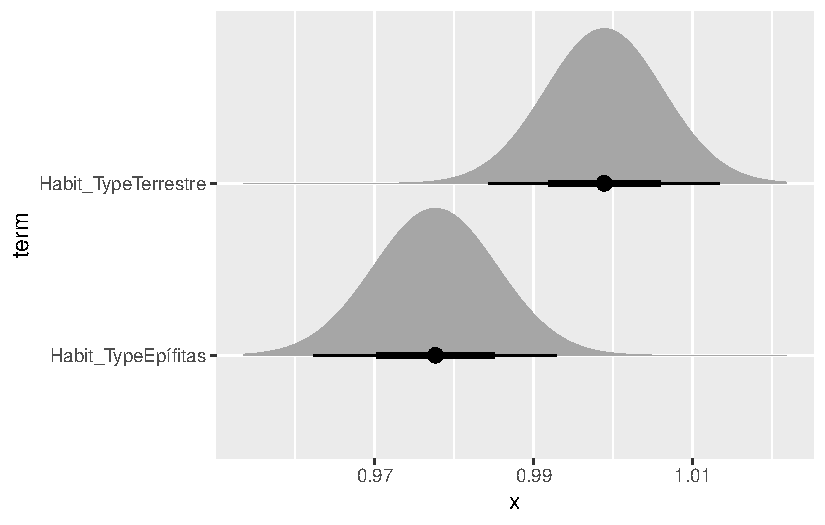
\includegraphics{120-Rage_orquideas_files/figure-pdf/Rage31-1.pdf}

La gráfica anterior puede ocultar la dispersión de los datos,
especialmente cuando hay sesgos. Para abordar esto, se pueden añadir los
datos originales a la figura. En este caso, se ha incorporado un símbolo
de barra \textbf{\textbar{}} por cada valor de lambda en la parte
inferior de la gráfica. Al observar esta nueva visualización, se nota
que la dispersión varía significativamente si se compara la
representación basada en el promedio y el error estándar con la
distribución real de los datos, representada por los
\textbf{\textbar{}}. Esta figura permite apreciar mejor tanto la
dispersión como la distribución de los datos. En comparación con la
gráfica anterior, esta ofrece una perspectiva más completa, destacando
los valores que se alejan del centro de la distribución.

\begin{Shaded}
\begin{Highlighting}[]
\NormalTok{ALL\_Lambdas }\SpecialCharTok{\%\textgreater{}\%}
  \FunctionTok{expand}\NormalTok{(Habit\_Type) }\SpecialCharTok{\%\textgreater{}\%}
  \FunctionTok{augment}\NormalTok{(model\_lambda, }\AttributeTok{newdata =}\NormalTok{ ., }\AttributeTok{se\_fit =} \ConstantTok{TRUE}\NormalTok{) }\SpecialCharTok{\%\textgreater{}\%}
  \FunctionTok{ggplot}\NormalTok{(}\FunctionTok{aes}\NormalTok{(}\AttributeTok{y =}\NormalTok{ Habit\_Type, }\AttributeTok{colour =}\NormalTok{ Habit\_Type)) }\SpecialCharTok{+}
  \FunctionTok{stat\_halfeye}\NormalTok{(}
    \FunctionTok{aes}\NormalTok{(}
      \AttributeTok{xdist =} \FunctionTok{dist\_student\_t}\NormalTok{(}
        \AttributeTok{df =} \FunctionTok{df.residual}\NormalTok{(model\_lambda),}
        \AttributeTok{mu =}\NormalTok{ .fitted,}
        \AttributeTok{sigma =}\NormalTok{ .se.fit}
\NormalTok{      )}
\NormalTok{    ),}
    \AttributeTok{scale =}\NormalTok{ .}\DecValTok{5}
\NormalTok{  ) }\SpecialCharTok{+}
  \FunctionTok{geom\_point}\NormalTok{(}
    \FunctionTok{aes}\NormalTok{(}\AttributeTok{x =}\NormalTok{ lambda),}
    \AttributeTok{data =}\NormalTok{ ALL\_Lambdas,}
    \AttributeTok{pch =} \StringTok{"|"}\NormalTok{,}
    \AttributeTok{size =} \DecValTok{2}\NormalTok{,}
    \AttributeTok{position =} \FunctionTok{position\_nudge}\NormalTok{(}\AttributeTok{y =} \SpecialCharTok{{-}}\NormalTok{.}\DecValTok{15}\NormalTok{)}
\NormalTok{  )}\SpecialCharTok{+}
  \FunctionTok{theme}\NormalTok{(}\AttributeTok{legend.position =} \FunctionTok{c}\NormalTok{(}\FloatTok{0.1}\NormalTok{, }\FloatTok{0.8}\NormalTok{)) }\SpecialCharTok{+}
  \FunctionTok{rlt\_style\_colour}\NormalTok{()}\SpecialCharTok{+}
  \FunctionTok{ylab}\NormalTok{(}\StringTok{""}\NormalTok{)}
\end{Highlighting}
\end{Shaded}

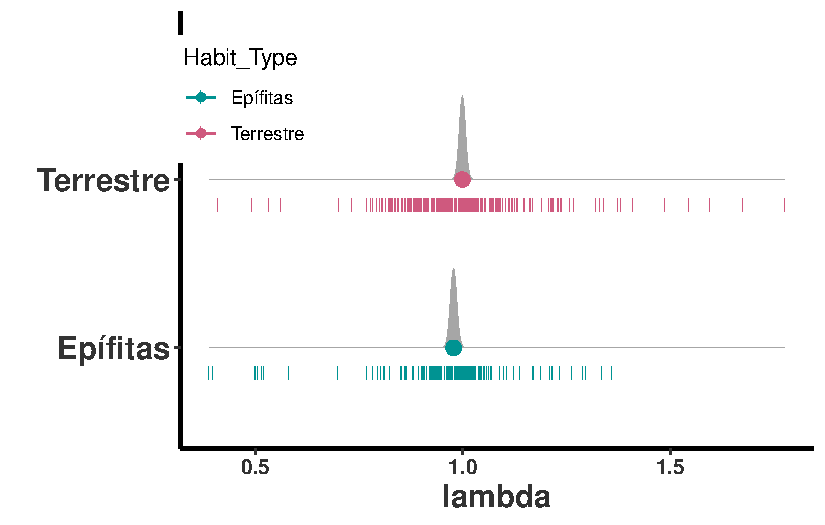
\includegraphics{120-Rage_orquideas_files/figure-pdf/Rage32-1.pdf}

\begin{center}\rule{0.5\linewidth}{0.5pt}\end{center}

\section{Mapa de distribución de los
estudios.}\label{mapa-de-distribuciuxf3n-de-los-estudios.}

La lista presentada corresponde a los datos extraídos de la base de
datos COMPADRE, complementados con información obtenida directamente de
los artículos científicos, con el objetivo de construir un mapa que
muestre dónde se han realizado estudios de dinámica poblacional.

Lamentablemente, COMPADRE aún carece de muchos datos y detalles
importantes que deberían incorporarse a su base. En esta sección, se
realizó una búsqueda específica de estudios sobre orquídeas dentro de
COMPADRE, extrayendo las coordenadas de latitud y longitud directamente
de los artículos originales.

En los casos en que no se encontraron coordenadas exactas, pero sí se
identificó el país o región del estudio, se utilizó Google Maps para
estimar las coordenadas aproximadas del sitio de muestreo. Cuando no fue
posible obtener ninguna información sobre la localización del estudio,
esos casos fueron excluidos del mapa.

Agradezco a Diana Molina Ozuma por su valiosa colaboración en la
búsqueda de las coordenadas de los sitios de estudio.

\begin{Shaded}
\begin{Highlighting}[]
\NormalTok{Orchid\_data\_DOI\_Diana\_3a }\OtherTok{\textless{}{-}} \FunctionTok{read\_excel}\NormalTok{(}\StringTok{"data/Orchid\_data\_DOI\_Diana\_3a.xlsx"}\NormalTok{)}
\end{Highlighting}
\end{Shaded}

\begin{Shaded}
\begin{Highlighting}[]
\NormalTok{Lat\_Long }\OtherTok{=}\NormalTok{ Orchid\_data\_DOI\_Diana\_3a }\SpecialCharTok{\%\textgreater{}\%}
  \FunctionTok{select}\NormalTok{(SpeciesAccepted, Lon, Lat, OrganismType) }\SpecialCharTok{|\textgreater{}}
  \FunctionTok{distinct}\NormalTok{(SpeciesAccepted, Lon, Lat, OrganismType)}

\CommentTok{\#write\_csv(Lat\_Long, "data/Orchid\_data\_DOI\_Diana\_3a.csv")}
\end{Highlighting}
\end{Shaded}

\begin{center}\rule{0.5\linewidth}{0.5pt}\end{center}

\subsection{Visualización de distribución
geospatial}\label{visualizaciuxf3n-de-distribuciuxf3n-geospatial}

Para representar la distribución geográfica de las orquídeas registradas
en la base de datos \texttt{COMPADRE}, se utilizó el paquete
\textbf{ggplot2}. En esta visualización, se emplea la función
\textbf{borders}, que incorpora los contornos de los países al mapa.
Esta función se basa en el paquete maps, el cual proporciona los datos
geográficos necesarios para delinear los límites nacionales, permitiendo
contextualizar espacialmente los puntos de muestreo.

\begin{Shaded}
\begin{Highlighting}[]
\NormalTok{ggplot2}\SpecialCharTok{::}\FunctionTok{ggplot}\NormalTok{(Lat\_Long, }\FunctionTok{aes}\NormalTok{(Lon, Lat, }\AttributeTok{colour =}\NormalTok{ OrganismType)) }\SpecialCharTok{+}
  \FunctionTok{annotation\_borders}\NormalTok{(}\AttributeTok{database =} \StringTok{"world"}\NormalTok{, }\AttributeTok{fill =} \StringTok{"grey80"}\NormalTok{, }\AttributeTok{col =} \ConstantTok{NA}\NormalTok{) }\SpecialCharTok{+}
  \FunctionTok{geom\_point}\NormalTok{(}\AttributeTok{size =} \FloatTok{1.0}\NormalTok{, }\AttributeTok{alpha =} \FloatTok{0.5}\NormalTok{)}\SpecialCharTok{+}
  \FunctionTok{theme}\NormalTok{(}\AttributeTok{legend.position =} \FunctionTok{c}\NormalTok{(}\FloatTok{0.15}\NormalTok{,}\FloatTok{0.2}\NormalTok{))}\SpecialCharTok{+}
  \FunctionTok{rlt\_style\_colour}\NormalTok{()}
\end{Highlighting}
\end{Shaded}

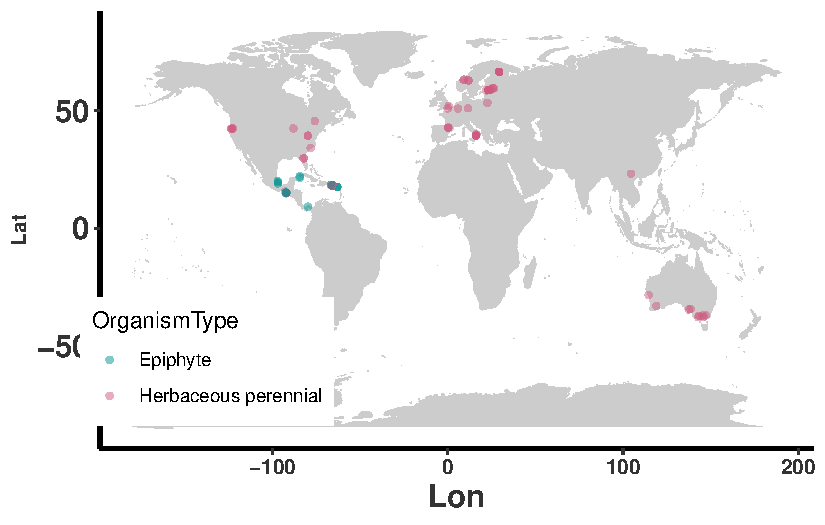
\includegraphics{120-Rage_orquideas_files/figure-pdf/Rage35-1.pdf}

\begin{Shaded}
\begin{Highlighting}[]
\CommentTok{\#ggsave("orchid\_map.jpg")}
\end{Highlighting}
\end{Shaded}

\begin{center}\rule{0.5\linewidth}{0.5pt}\end{center}

\section{Mapa de distribución interactivo con
Leaflet}\label{mapa-de-distribuciuxf3n-interactivo-con-leaflet}

Se utilizó el paquete Leaflet para crear un mapa interactivo que muestra
los sitios de muestreo de las especies de orquídeas estudiadas en campo.
Este enfoque permite explorar visualmente la distribución geográfica de
las poblaciones incluidas en los estudios.

El mapa revela una marcada disparidad en los sitios de muestreo entre
los dos tipos de orquídeas. Las poblaciones marcadas en rojo
corresponden a especies epífitas, mientras que las azules representan
especies terrestres. Se observa que las especies terrestres están
principalmente distribuidas en Europa y América del Norte, con escasa
representación en Asia y ninguna en África. Por otro lado, las especies
epífitas se concentran en el Caribe y América Central (especialmente
México), sin presencia en África, Asia ni Australia.

Además, el mapa es interactivo y permite hacer zoom para examinar áreas
específicas con mayor detalle. Presiona sobre los puntos para obtener
información adicional sobre el nombre científico de la especie
muestreada en este sitio.

\begin{Shaded}
\begin{Highlighting}[]
\NormalTok{PointUsePalette }\OtherTok{\textless{}{-}}\NormalTok{ leaflet}\SpecialCharTok{::}\FunctionTok{colorFactor}\NormalTok{(}
  \AttributeTok{palette =} \FunctionTok{c}\NormalTok{(}\StringTok{"\#009392"}\NormalTok{, }\StringTok{"\#CF597E"}\NormalTok{),}
  \AttributeTok{domain =} \FunctionTok{c}\NormalTok{(}\StringTok{"Epiphyte"}\NormalTok{, }\StringTok{"Herbaceous perennial"}\NormalTok{)}
\NormalTok{) }\CommentTok{\# para asignar los colores a los factores (clase de Vida)}

\NormalTok{Orchid\_map }\OtherTok{=} \FunctionTok{leaflet}\NormalTok{(Lat\_Long) }\SpecialCharTok{\%\textgreater{}\%} \CommentTok{\# los datos}
  \FunctionTok{addTiles}\NormalTok{() }\SpecialCharTok{\%\textgreater{}\%}
  \FunctionTok{addCircleMarkers}\NormalTok{(}
    \AttributeTok{lng =} \SpecialCharTok{\textasciitilde{}}\NormalTok{Lon, }\CommentTok{\# la longitud}
    \AttributeTok{lat =} \SpecialCharTok{\textasciitilde{}}\NormalTok{Lat, }\CommentTok{\# la latitud}
    \AttributeTok{radius =} \DecValTok{2}\NormalTok{, }\CommentTok{\# el tamaño del punto}
    \AttributeTok{color =} \SpecialCharTok{\textasciitilde{}} \FunctionTok{PointUsePalette}\NormalTok{(OrganismType), }\CommentTok{\# Para colorear los puntos por el tipo clase de vida}
    \AttributeTok{popup =} \SpecialCharTok{\textasciitilde{}} \FunctionTok{paste0}\NormalTok{(}\StringTok{"\textless{}I\textgreater{}"}\NormalTok{, SpeciesAccepted, }\StringTok{"\textless{}/I\textgreater{}"}\NormalTok{) }\CommentTok{\# para poner los nombres científicos en itálicos}
\NormalTok{  )}

\NormalTok{Orchid\_map}
\end{Highlighting}
\end{Shaded}

\begin{verbatim}
file:////private/var/folders/3k/1ft37x9130vdbz21tw1497x40000gn/T/RtmpLaZkwn/file10509ec0c9c6/widget1050912feedbb.html screenshot completed
\end{verbatim}

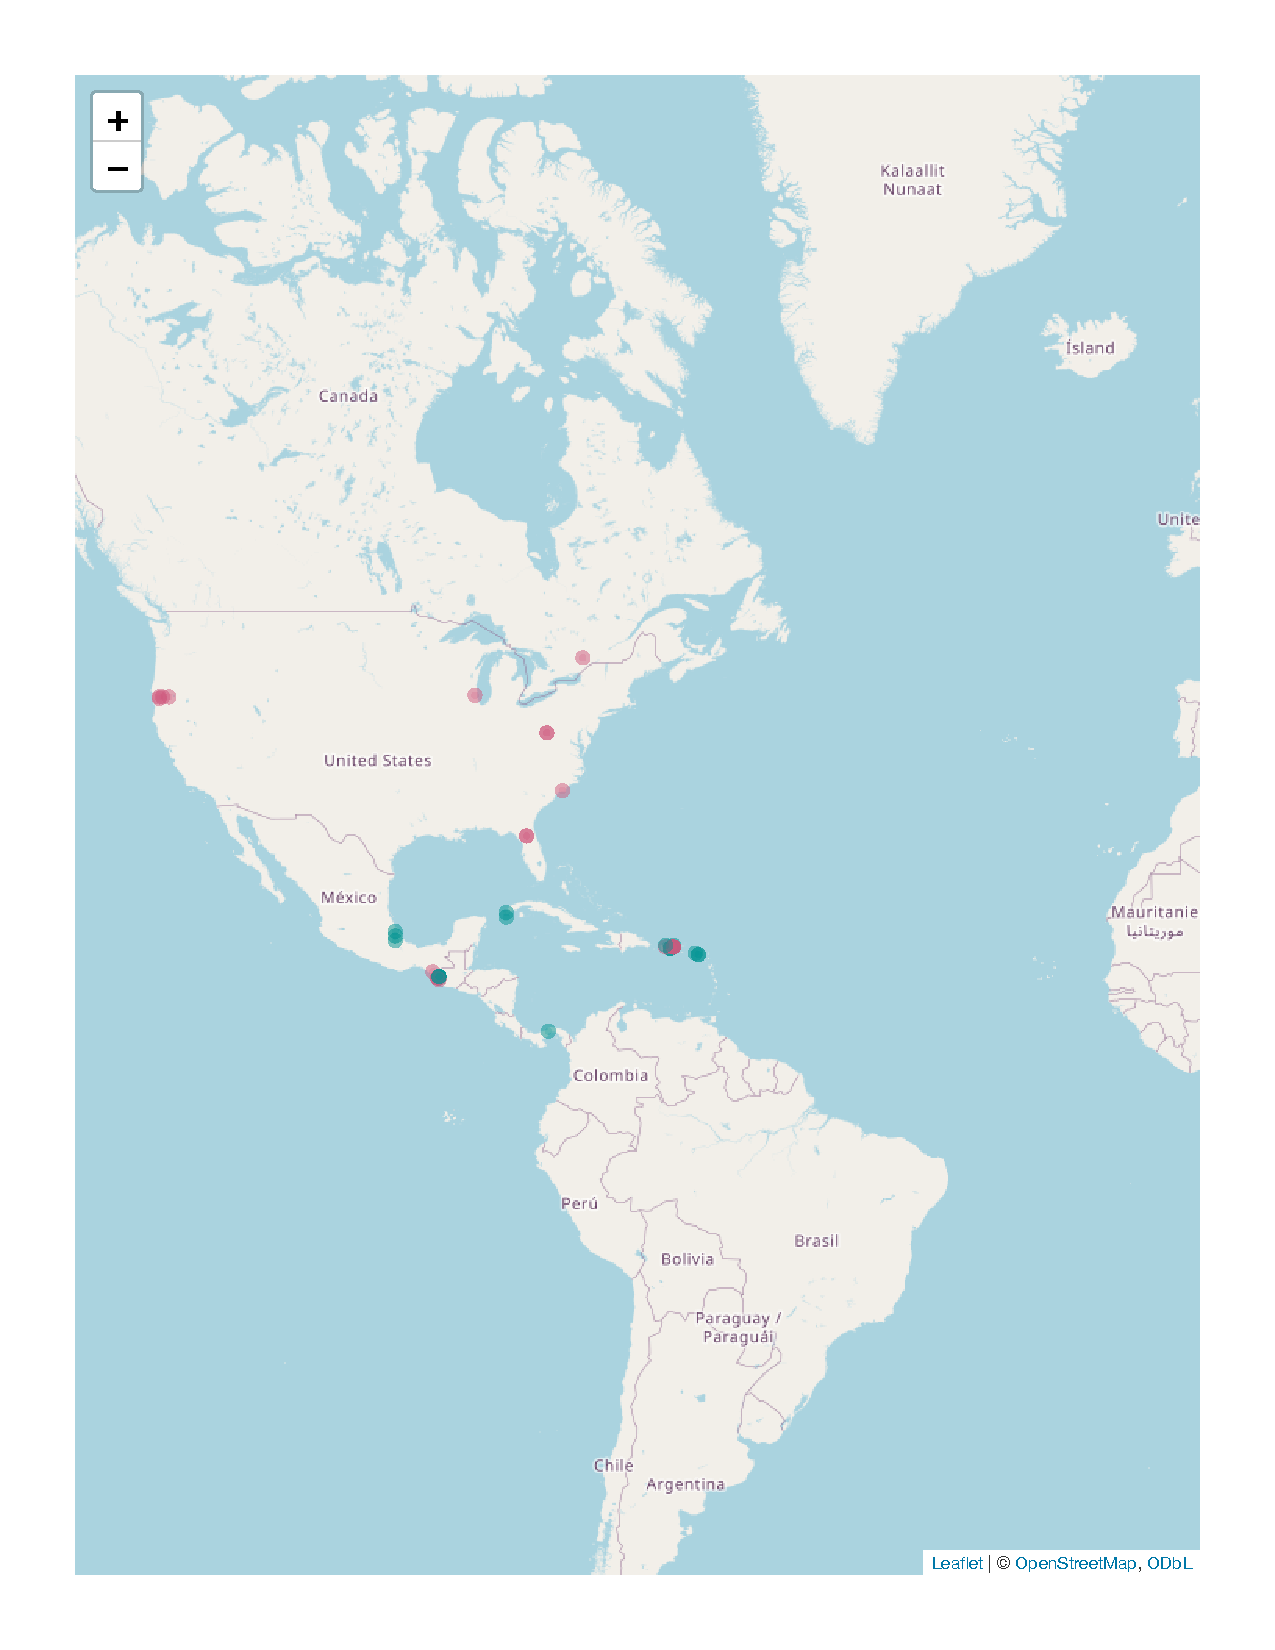
\includegraphics{120-Rage_orquideas_files/figure-pdf/Rage36-1.pdf}

\begin{Shaded}
\begin{Highlighting}[]
\CommentTok{\# htmltools::save\_html(Orchid\_map, file = "Orchid\_map.html") \# El script para crear un archivo aparte del mapa}
\end{Highlighting}
\end{Shaded}

\begin{center}\rule{0.5\linewidth}{0.5pt}\end{center}

http://127.0.0.1:29465/rmd\_output/1/compadre\_orchid-ppm-y-su-uso.html

Revisión RLT:

Sept 15, 2024

Jan 20, 2025

\phantomsection\label{refs}
\begin{CSLReferences}{1}{0}
\bibitem[\citeproctext]{ref-tremblay2001gene}
Tremblay R, Ackerman J. 2001. Gene flow and effective population size in
\emph{{L}epanthes} ({O}rchidaceae): A case for genetic drift.
\emph{Biological Journal of the Linnean Society} 72:47--62. DOI:
\href{https://doi.org/10.1006/bijl.2000.0485}{10.1006/bijl.2000.0485}.

\bibitem[\citeproctext]{ref-tremblay2014bayesian}
Tremblay R, McCarthy MA. 2014. Bayesian estimates of transition
probabilities in seven small lithophytic orchid populations: Maximizing
data availability from many small samples. \emph{PLoS One} 9:e102859.

\end{CSLReferences}


\backmatter


\end{document}
